\documentclass[a4paper,10pt]{article}
\usepackage[utf8]{inputenc}
\usepackage[T1]{fontenc}
\usepackage[french]{babel}
\usepackage[top=0.7cm, bottom=0.7cm, left=0.7cm, right=0.7cm]{geometry}
\usepackage{multicol}
\usepackage{xcolor}
\usepackage{booktabs}
\usepackage{tabularx}
\usepackage{amsmath, amssymb}
\usepackage{enumitem}
\usepackage{hyperref}
\usepackage{tcolorbox}
\usepackage{lmodern}
\usepackage{graphicx}
\graphicspath{{../../imgs/}{../imgs/}{imgs/}}

\newcommand{\code}[1]{\texttt{\footnotesize #1}}
\newcommand{\tech}[1]{\textbf{\textcolor{OceanMedium}{#1}}}
\newcommand{\succw}[1]{\textbf{\textcolor{OceanGreen}{#1}}}
\newcommand{\alertw}[1]{\textbf{\textcolor{OceanCoral}{#1}}}

\pagestyle{empty}
\setlength{\columnsep}{8pt}
\setlist{nosep, leftmargin=9pt}

% Couleurs marines
\definecolor{OceanDeep}{HTML}{0A2240}
\definecolor{OceanMedium}{HTML}{0E4D7A}
\definecolor{OceanCyan}{HTML}{00A8B5}
\definecolor{OceanCoral}{HTML}{EF4444}
\definecolor{OceanGreen}{HTML}{10B981}
\definecolor{LightBg}{HTML}{F8FAFC}
\hypersetup{colorlinks=true, urlcolor=OceanMedium, linkcolor=OceanMedium}

\tcbset{
  colback=LightBg,
  colframe=OceanMedium,
  coltitle=white,
  fonttitle=\bfseries\scriptsize,
  boxrule=0.6pt,
  arc=2pt,
  left=2.5pt, right=2.5pt, top=2pt, bottom=2pt,
  boxsep=1.2pt
}

\begin{document}

% ==============================================================================
% PAGE 1 : VECTEURS, MECATRONIQUE, ENCEINTES & ENERGIE EMBARQUEE (RECTO)
% ==============================================================================
\begin{center}
  {\small\bfseries\textcolor{OceanDeep}{ANF ArchiDrone 2026 --- Réseaux Drone\&Cap' \& 2RM (Réseau Métier Roboticien et Mécatronicien)}} \\
  \vspace{1pt}
  {\large\bfseries\textcolor{OceanMedium}{Mémento Technique : Vecteurs Marins, Caissons, Énergie \& Pénétrateurs}} \\
  \vspace{1pt}
  {\scriptsize\textit{Formateur : Quentin Brateau --- 04 Novembre 2026 --- Matériel réel BlueRobotics, actionneurs, caissons 3"/4", WLP-JPT \& batteries}}
\end{center}
\vspace{-9pt}
\hrule height 0.8pt
\vspace{2pt}

\begin{multicols}{2}

% BLOC 1 : TYPOLOGIE DES VECTEURS ET ECOSYSTEME MARCHE
\begin{tcolorbox}[title={1. Typologie des Vecteurs : ROV, Micro-AUV \& ASV}]
  \begin{center}
    \resizebox{\linewidth}{!}{%
    \begin{tabular}{ccc}
      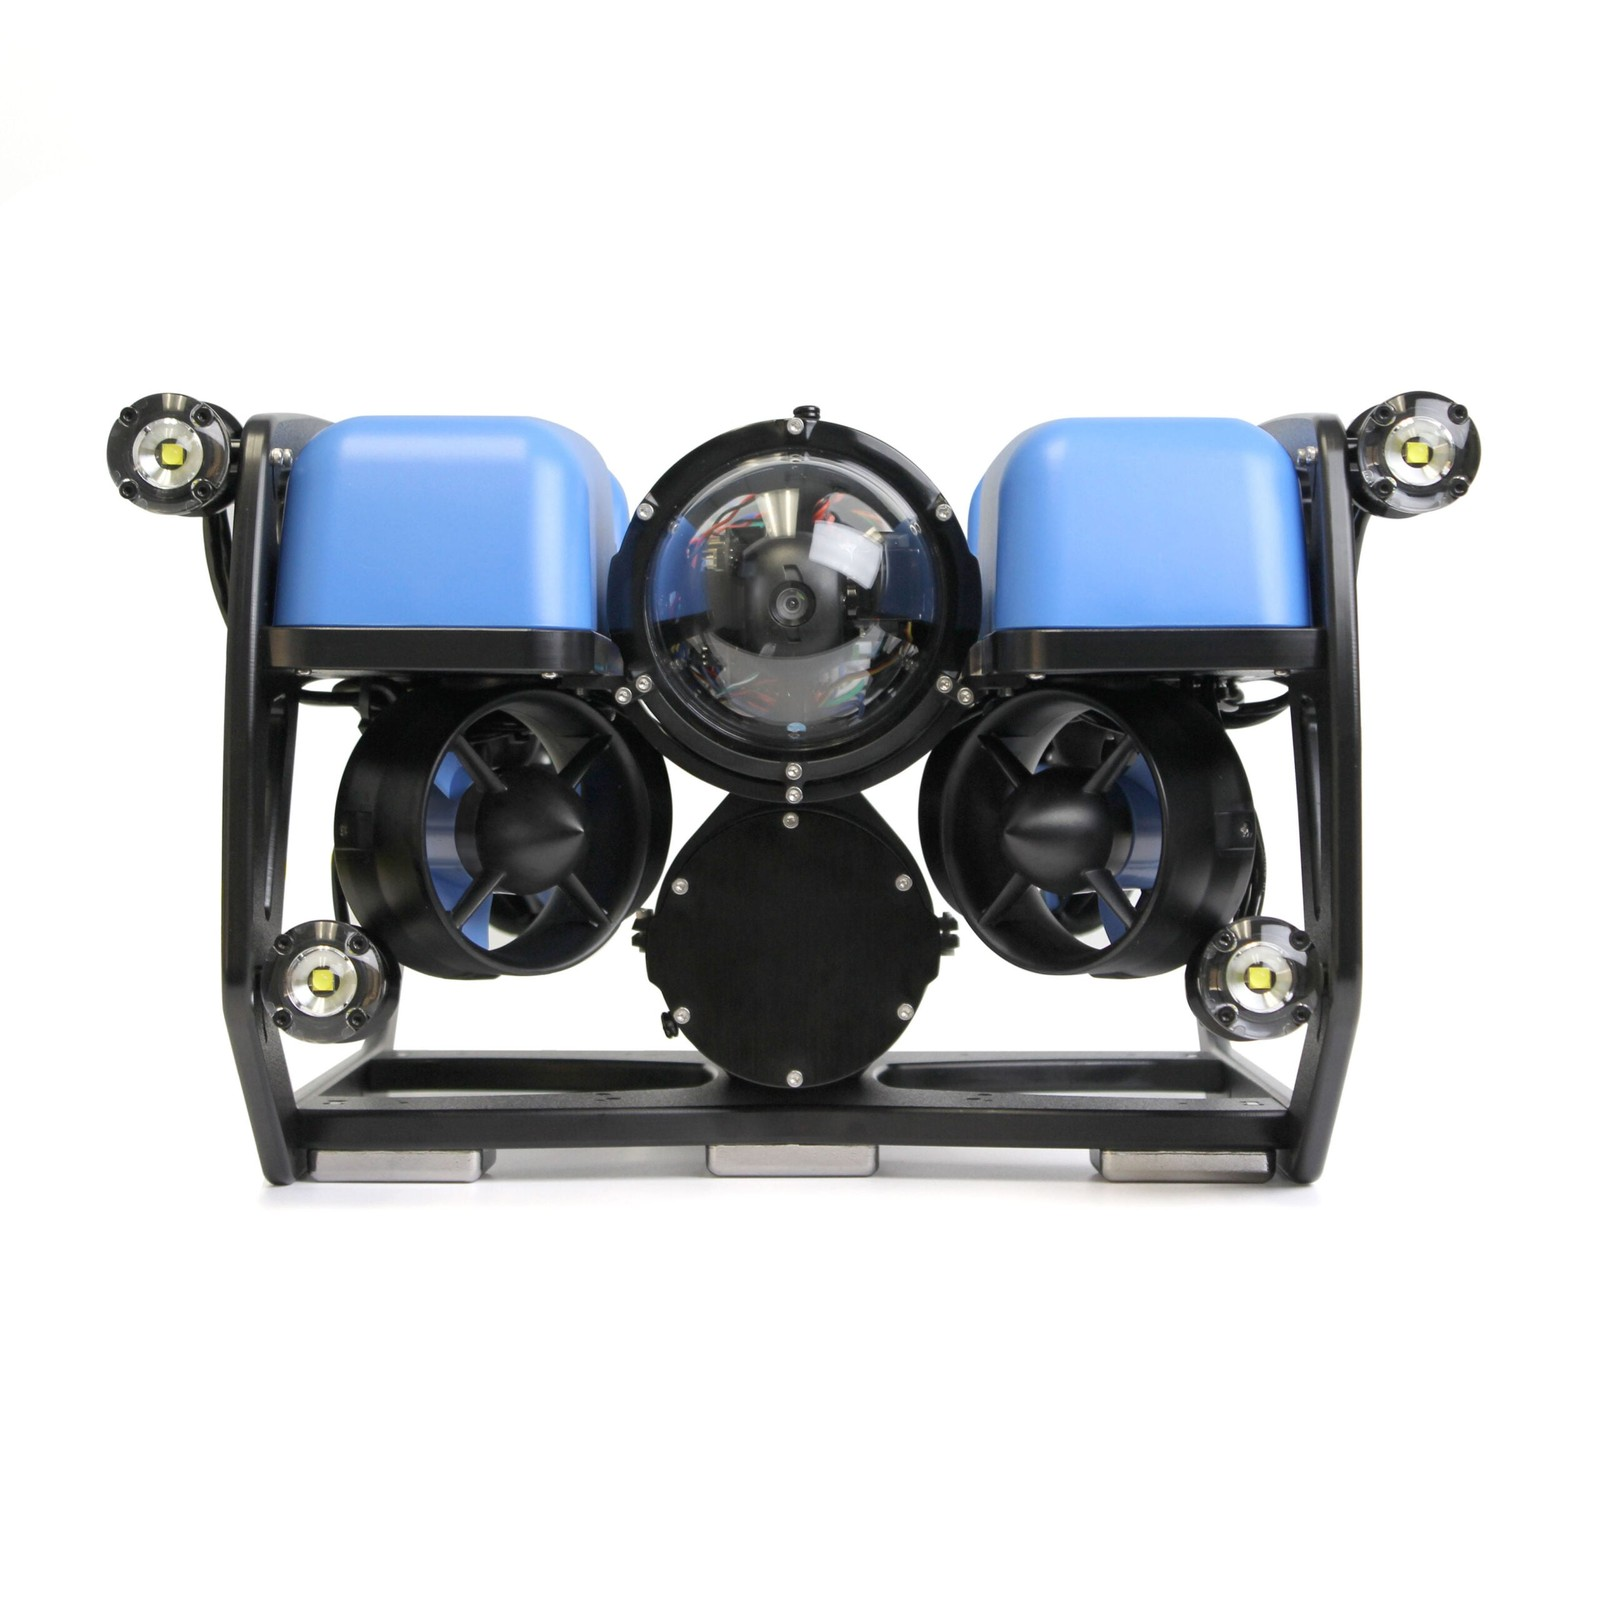
\includegraphics[height=1.25cm, keepaspectratio]{bluerov2.jpg} &
      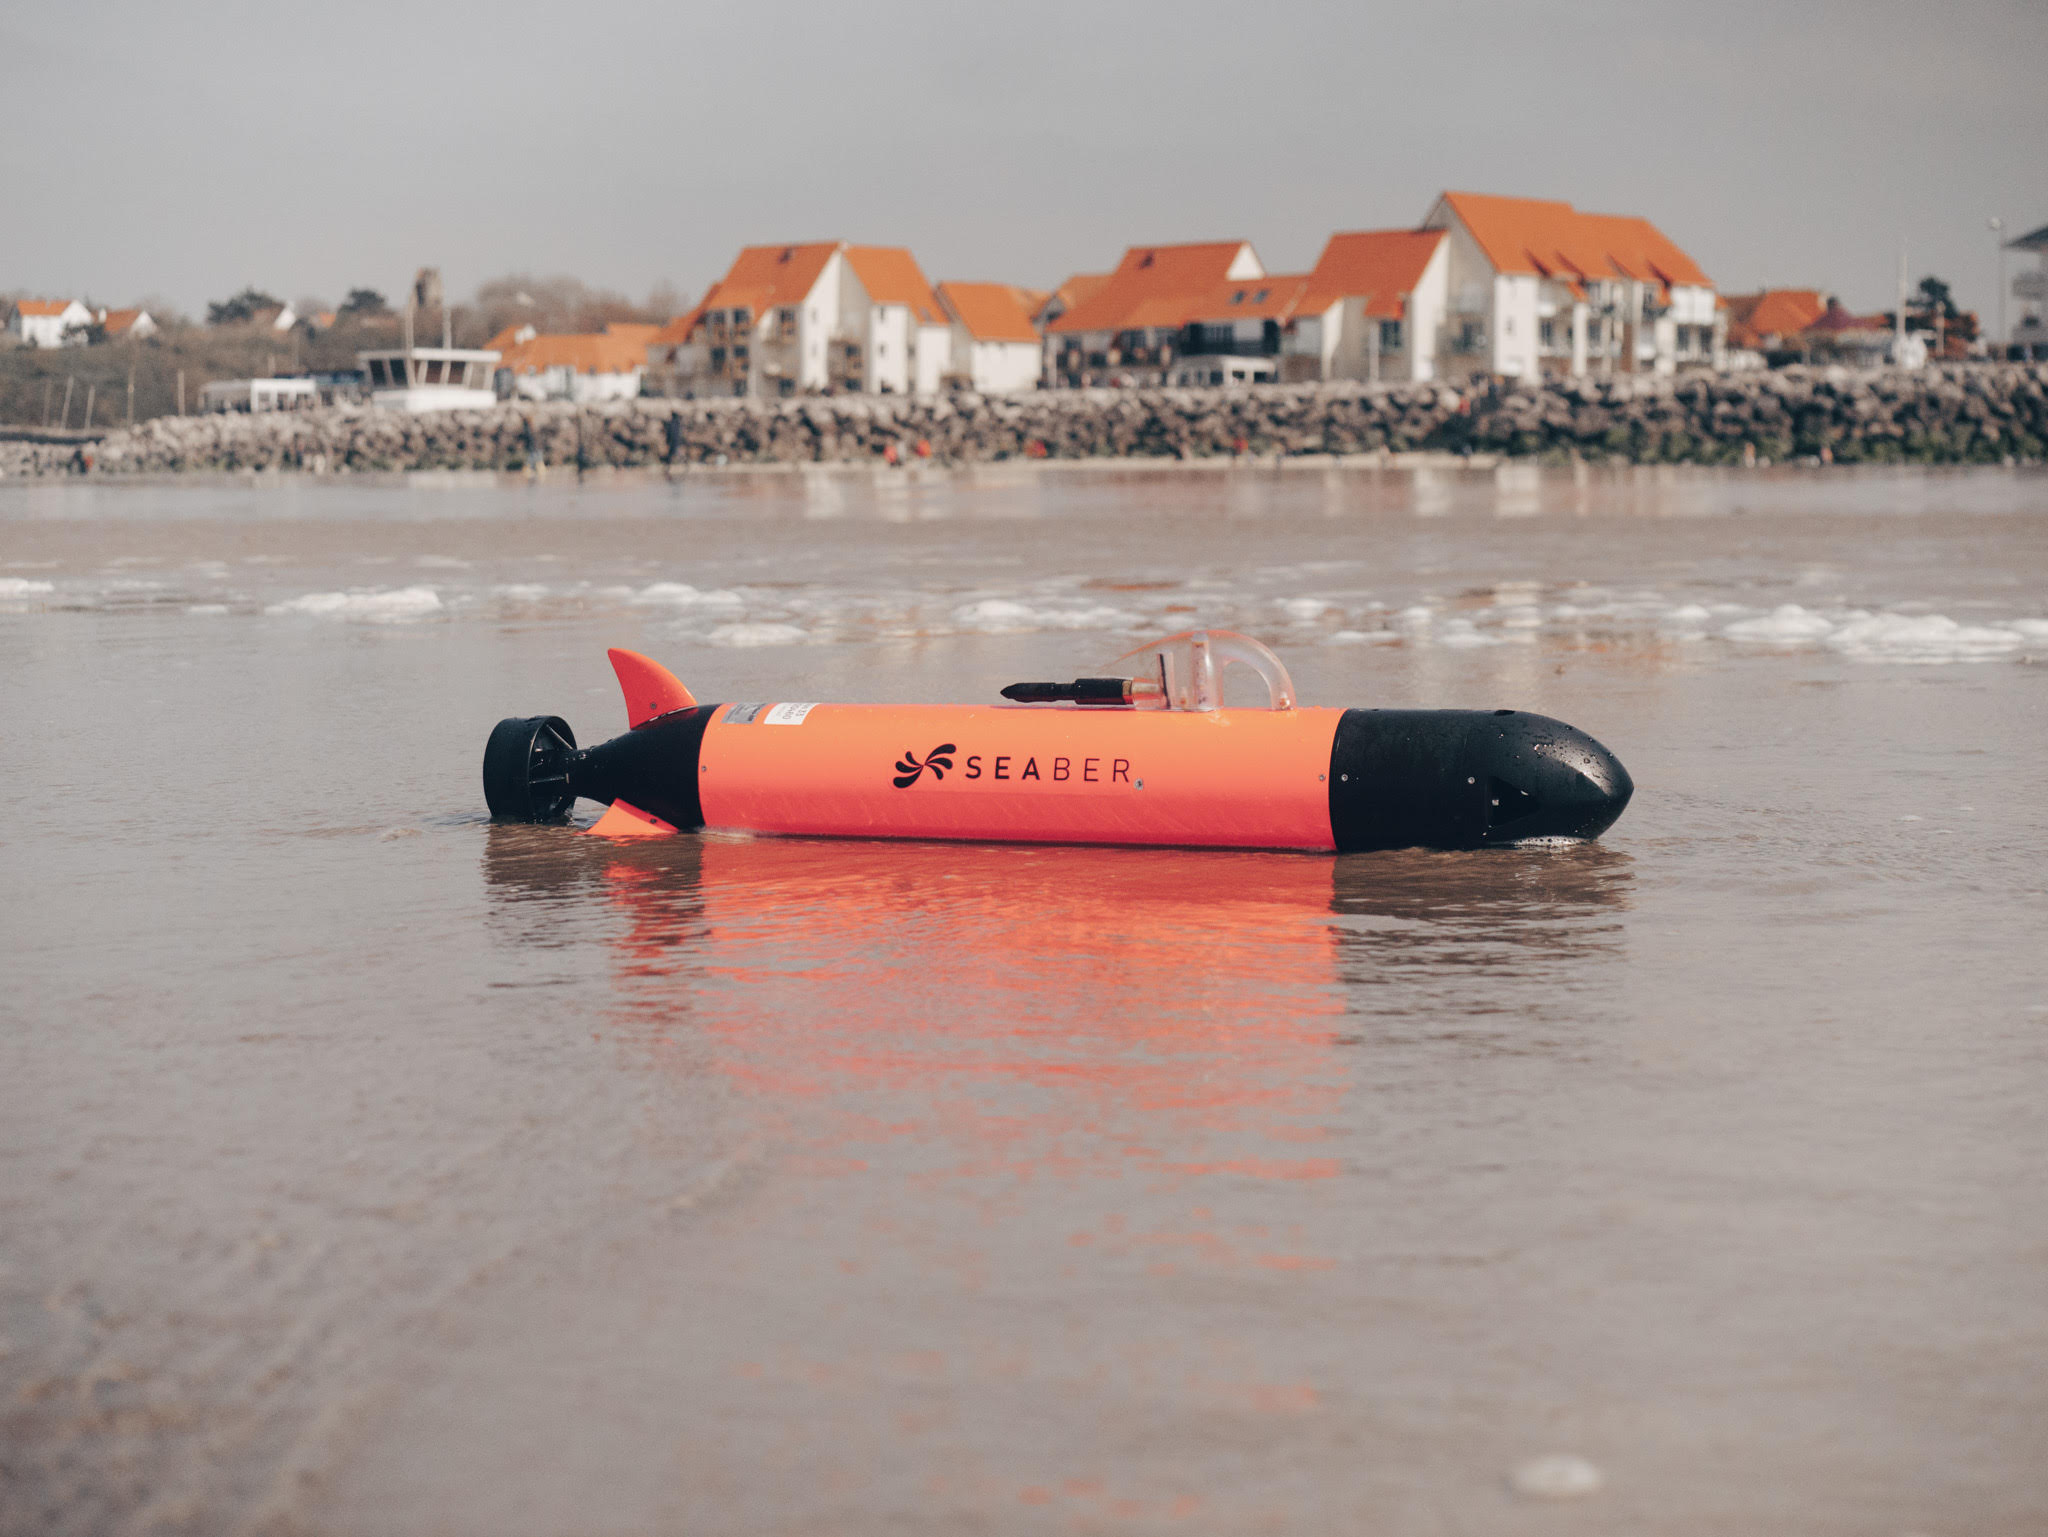
\includegraphics[height=1.25cm, keepaspectratio]{seaber_yuco.jpg} &
      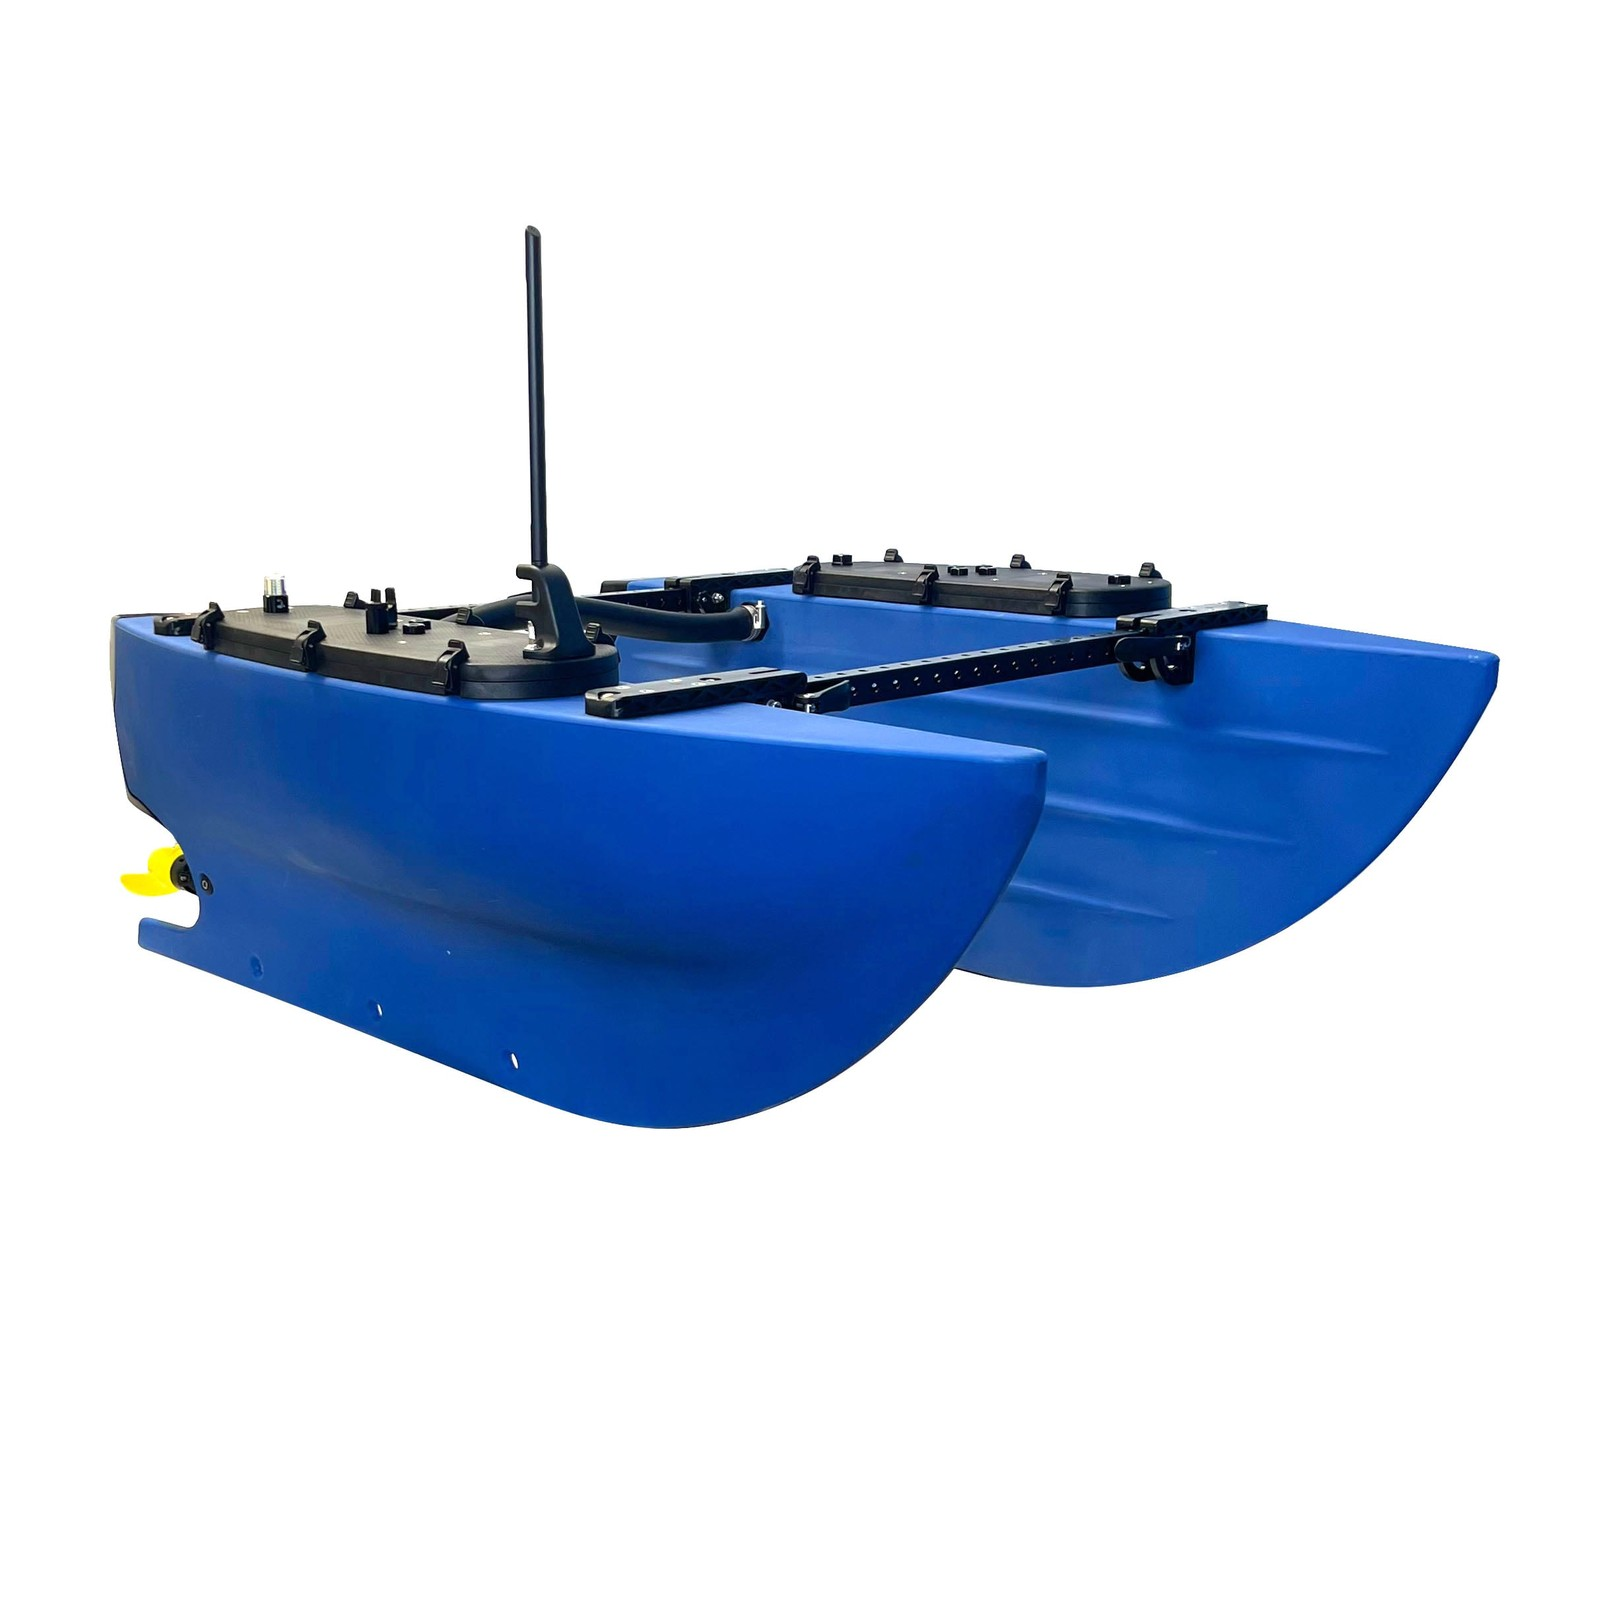
\includegraphics[height=1.25cm, keepaspectratio]{blueboat.jpg} \\
      \textbf{ROV : BlueROV2 (US)} &
      \textbf{Micro-AUV : YUCO (FR)} &
      \textbf{ASV : BlueBoat (US)}
    \end{tabular}%
    }
  \end{center}
  \scriptsize
  \begin{itemize}
    \item \textbf{ROV (BlueROV2 Heavy)} : filaire ombilical Fathom-X ($100\,\text{Mbps}$). 6 DDL, stationnaire précis, vidéo benthique HD, prélèvements pince. Budget équipé : $\approx \mathbf{8\text{--}15\,\text{k€}}$ (vs $>40\,\text{k€}$ ind.).
    \item \textbf{Micro-AUV (Seaber YUCO)} : autonome sans fil ($<10\,\text{kg}$, $\approx 1\,\text{m}$, $300\,\text{m}$). Navigation INX/DVL, profils CTD yo-yo, sonar latéral. Budget équipé : $\approx \mathbf{35\text{--}70\,\text{k€}}$ (vs $>200\,\text{k€}$ lourd).
    \item \textbf{ASV (BlueBoat)} : catamaran surface, tirant d'eau $15\,\text{cm}$, GNSS RTK Centipede, bathymétrie monofaisceau Ping ou multi Cerulean. Budget équipé : $\approx \mathbf{7\text{--}18\,\text{k€}}$ (vs $>50\,\text{k€}$ ind.).
    \item \textbf{Acteurs \& Revendeurs FR} : constructeurs BlueRobotics (US), Seaber (FR - Lorient), RTSYS (FR), Water Linked (NO). Revendeurs commandes publiques CNRS : \textbf{SyERA} (Toulon), \textbf{ROV Expert} (Béziers), \textbf{Subsea Tech} (Marseille).
  \end{itemize}
\end{tcolorbox}

% BLOC 2 : ACTIONNEURS REELS
\begin{tcolorbox}[title={2. Actionneurs Marins : T200, T500 \& Servos / Pinces}]
  \begin{center}
    \resizebox{\linewidth}{!}{%
    \begin{tabular}{ccc}
      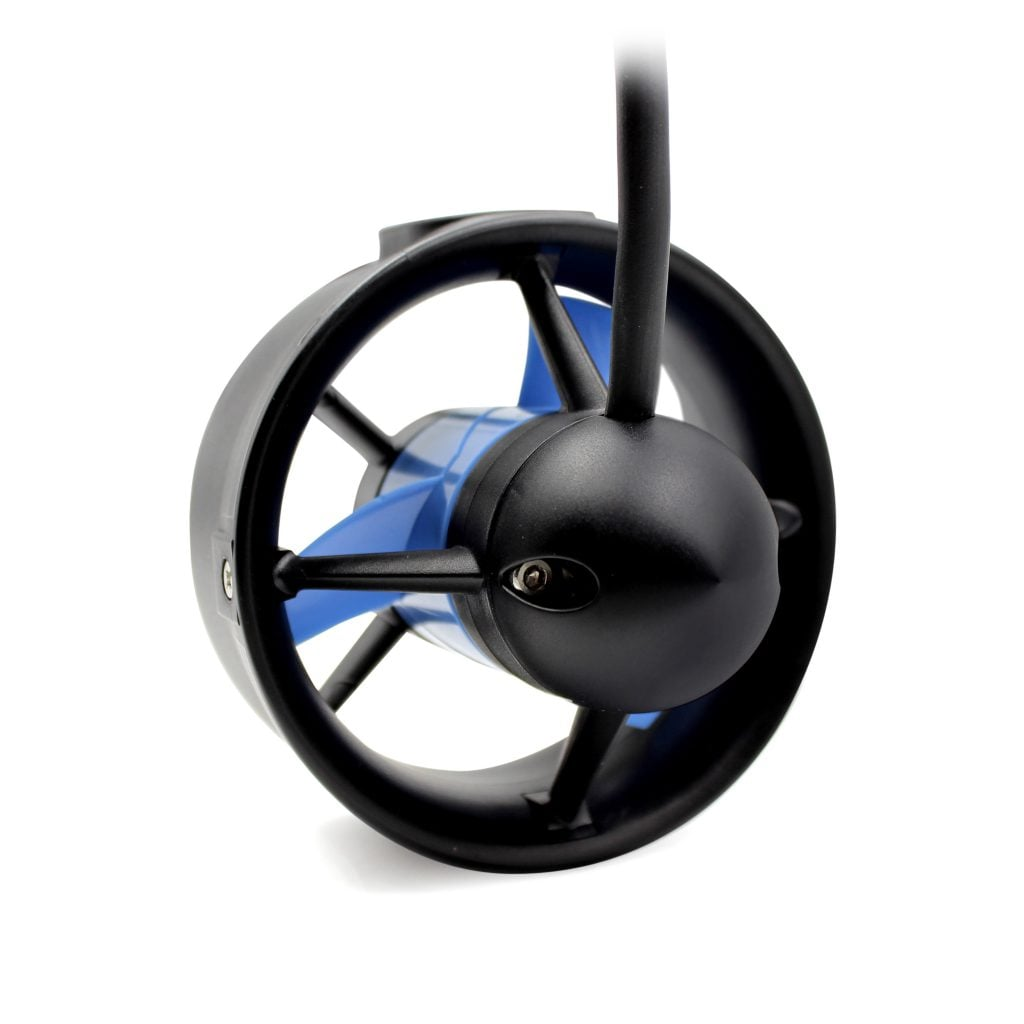
\includegraphics[height=1.35cm, keepaspectratio]{t200_thruster.png} &
      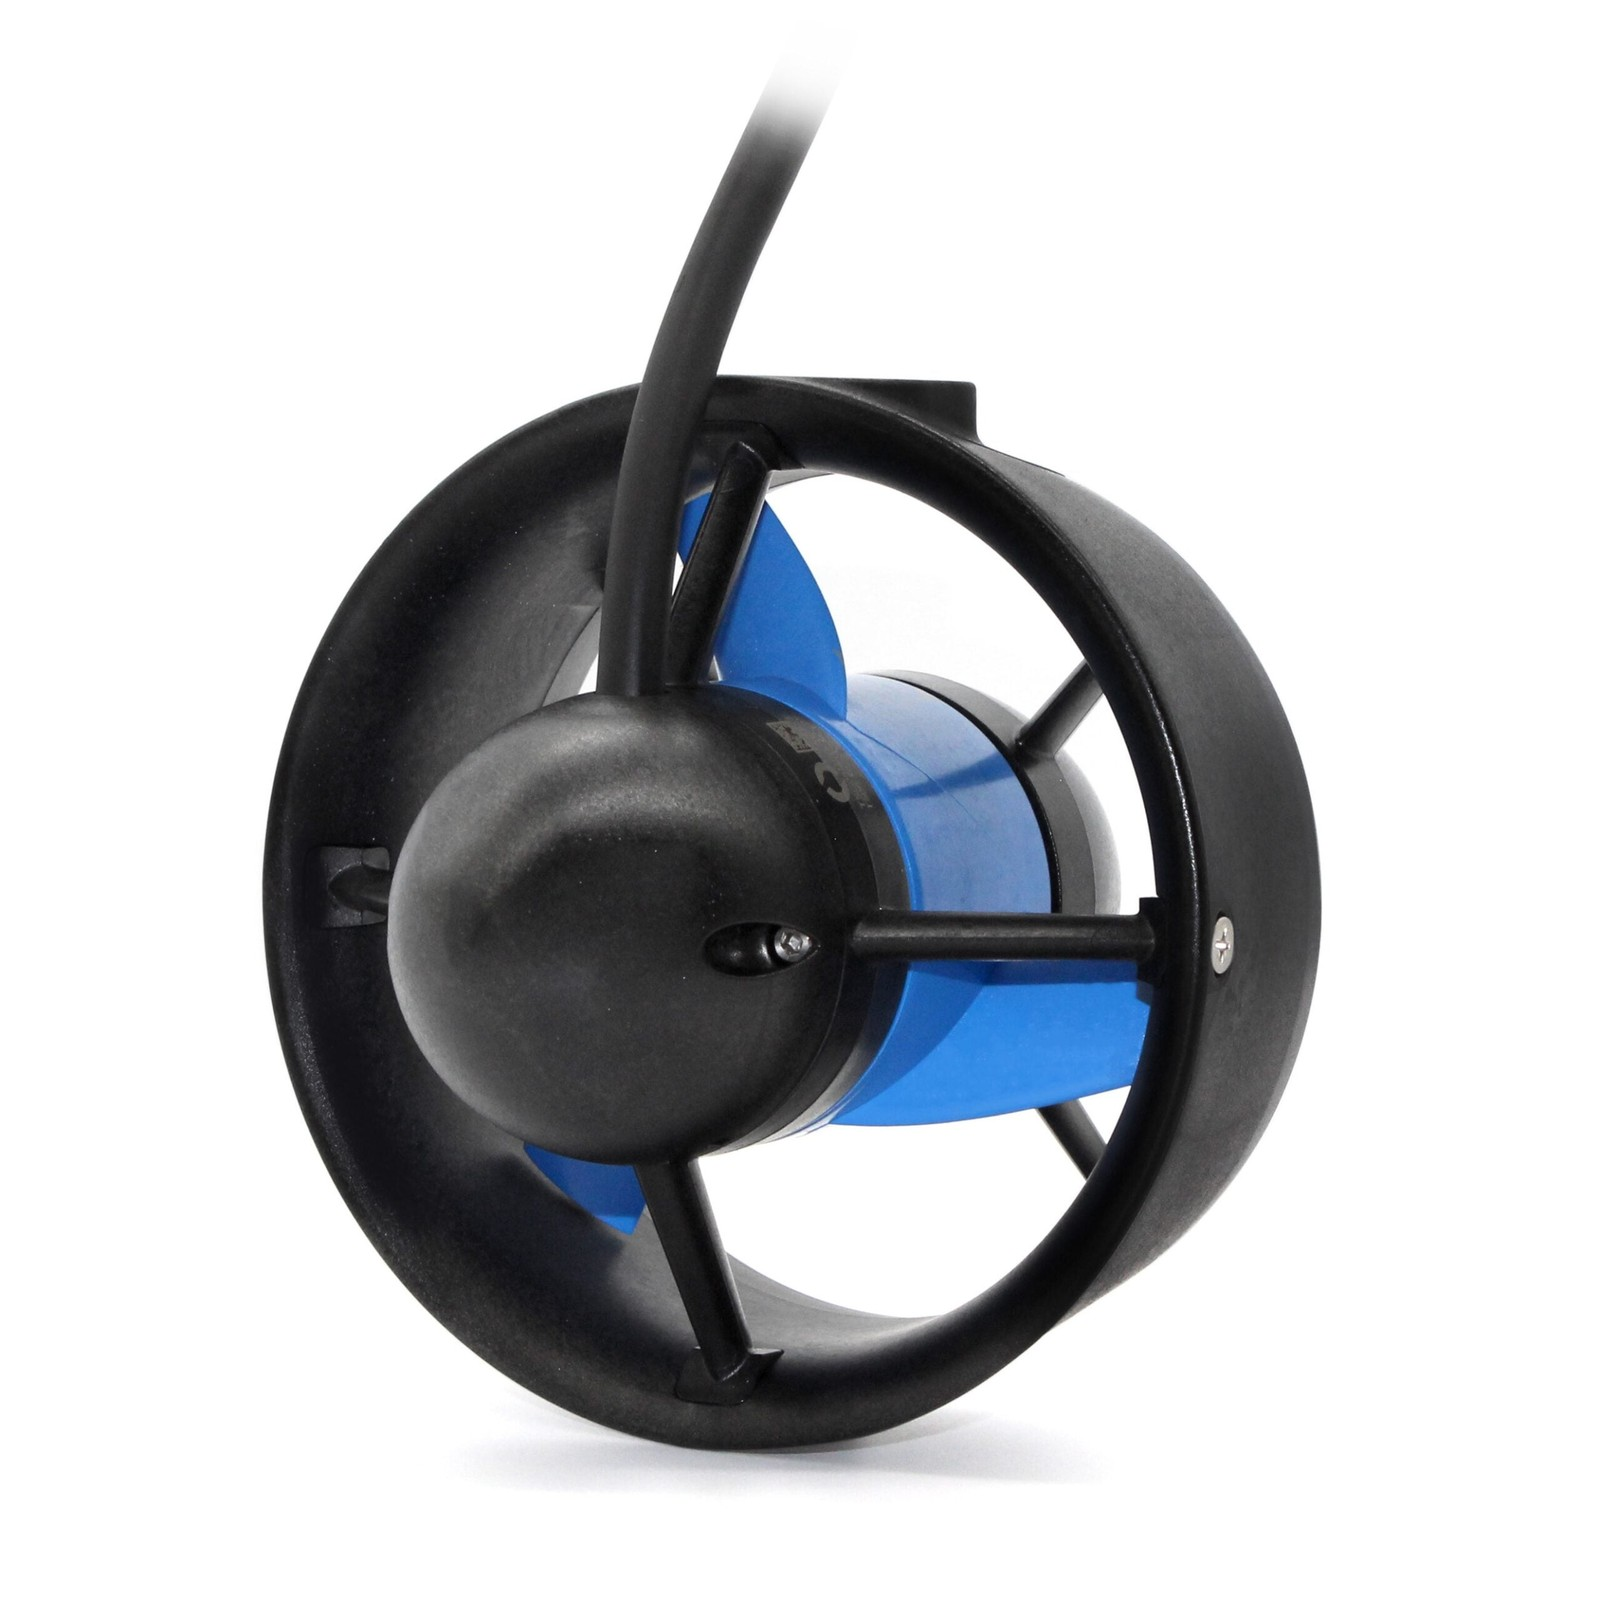
\includegraphics[height=1.35cm, keepaspectratio]{t500_thruster.jpg} &
      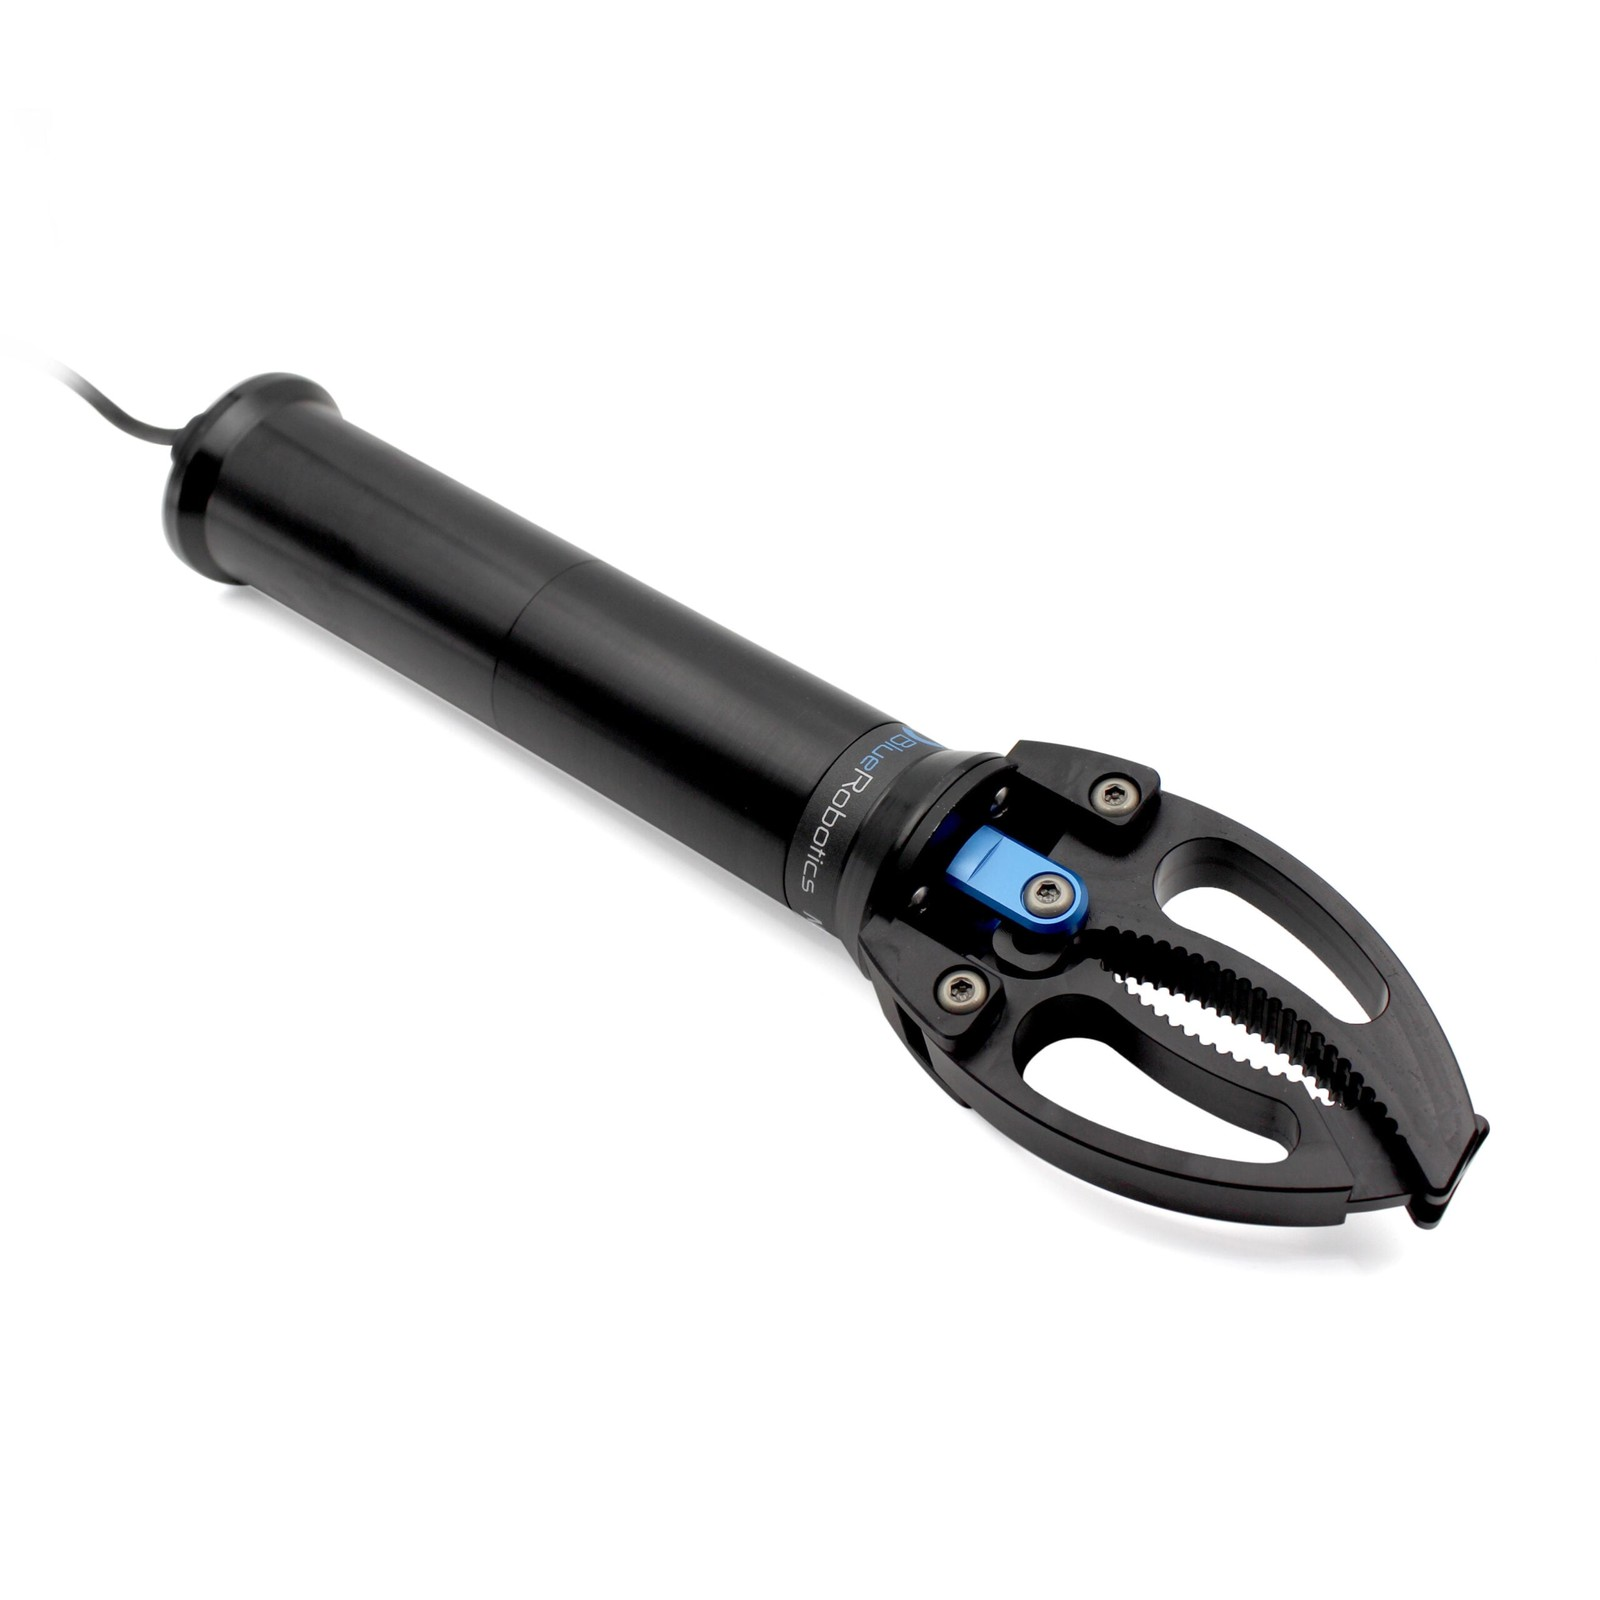
\includegraphics[height=1.35cm, keepaspectratio]{newton_gripper.jpg} \\
      \textbf{T200 ($5.25\,\text{kgf}$)} &
      \textbf{T500 ($16.1\,\text{kgf}$)} &
      \textbf{Pince Newton ($97\,\text{N}$)}
    \end{tabular}%
    }
  \end{center}
  \scriptsize
  \begin{itemize}
    \item \textbf{T200 Thruster} : moteur brushless noyé (*flooded*), stator surmoulé sous résine époxy, paliers PEEK autolubrifiants (zéro roulement métallique). Poussée $5.25\,\text{kgf}$, contrôleur Basic ESC 500 ($50\,\text{A}$).
    \item \textbf{T500 Thruster} : forte poussée ($16.1\,\text{kgf}$, $3\times$ T200), tension $24\,\text{V}$ pour gros AUVs et bateaux rapides.
    \item \textbf{Pince Newton \& Servos étanches} : actionneur linéaire submersible à $300\,\text{m}$, commande servo PWM standard ($1.1\text{--}1.9\,\text{ms}$), force $97\,\text{N}$.
  \end{itemize}
\end{tcolorbox}

% BLOC 3 : CALCULATEURS EMBARQUES & CAPTEURS DE SURETE
\begin{tcolorbox}[title={3. Calculateurs \& Capteurs de Sûreté Véhicule}]
  \begin{center}
    \resizebox{\linewidth}{!}{%
    \begin{tabular}{cccc}
      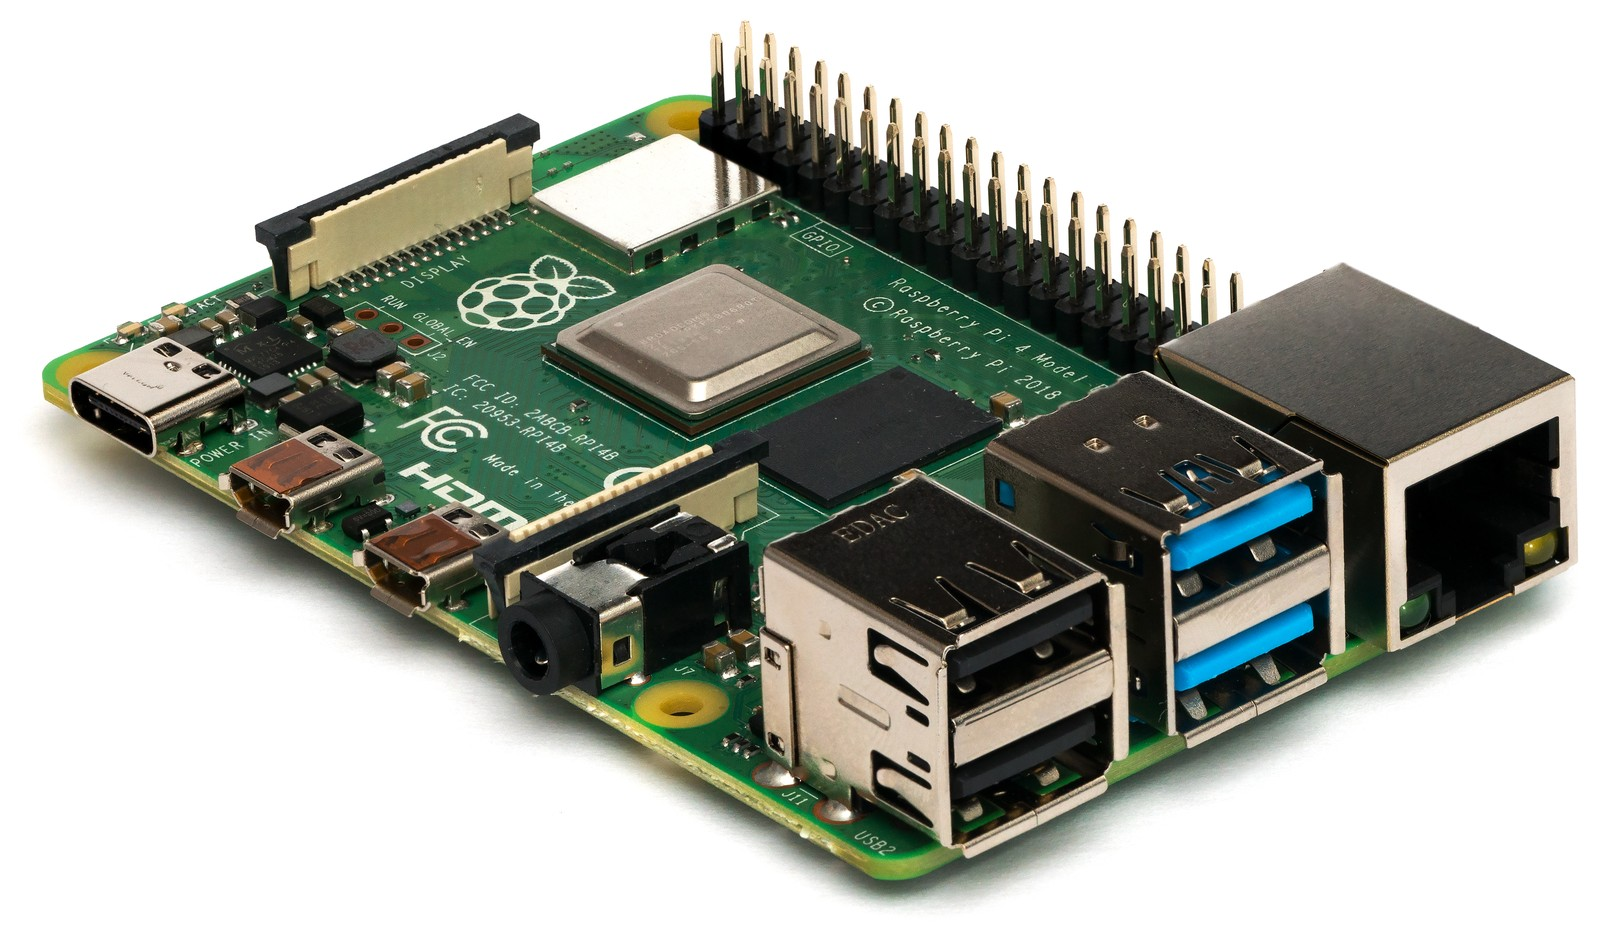
\includegraphics[height=1.25cm, keepaspectratio]{raspberry_pi_4.jpg} &
      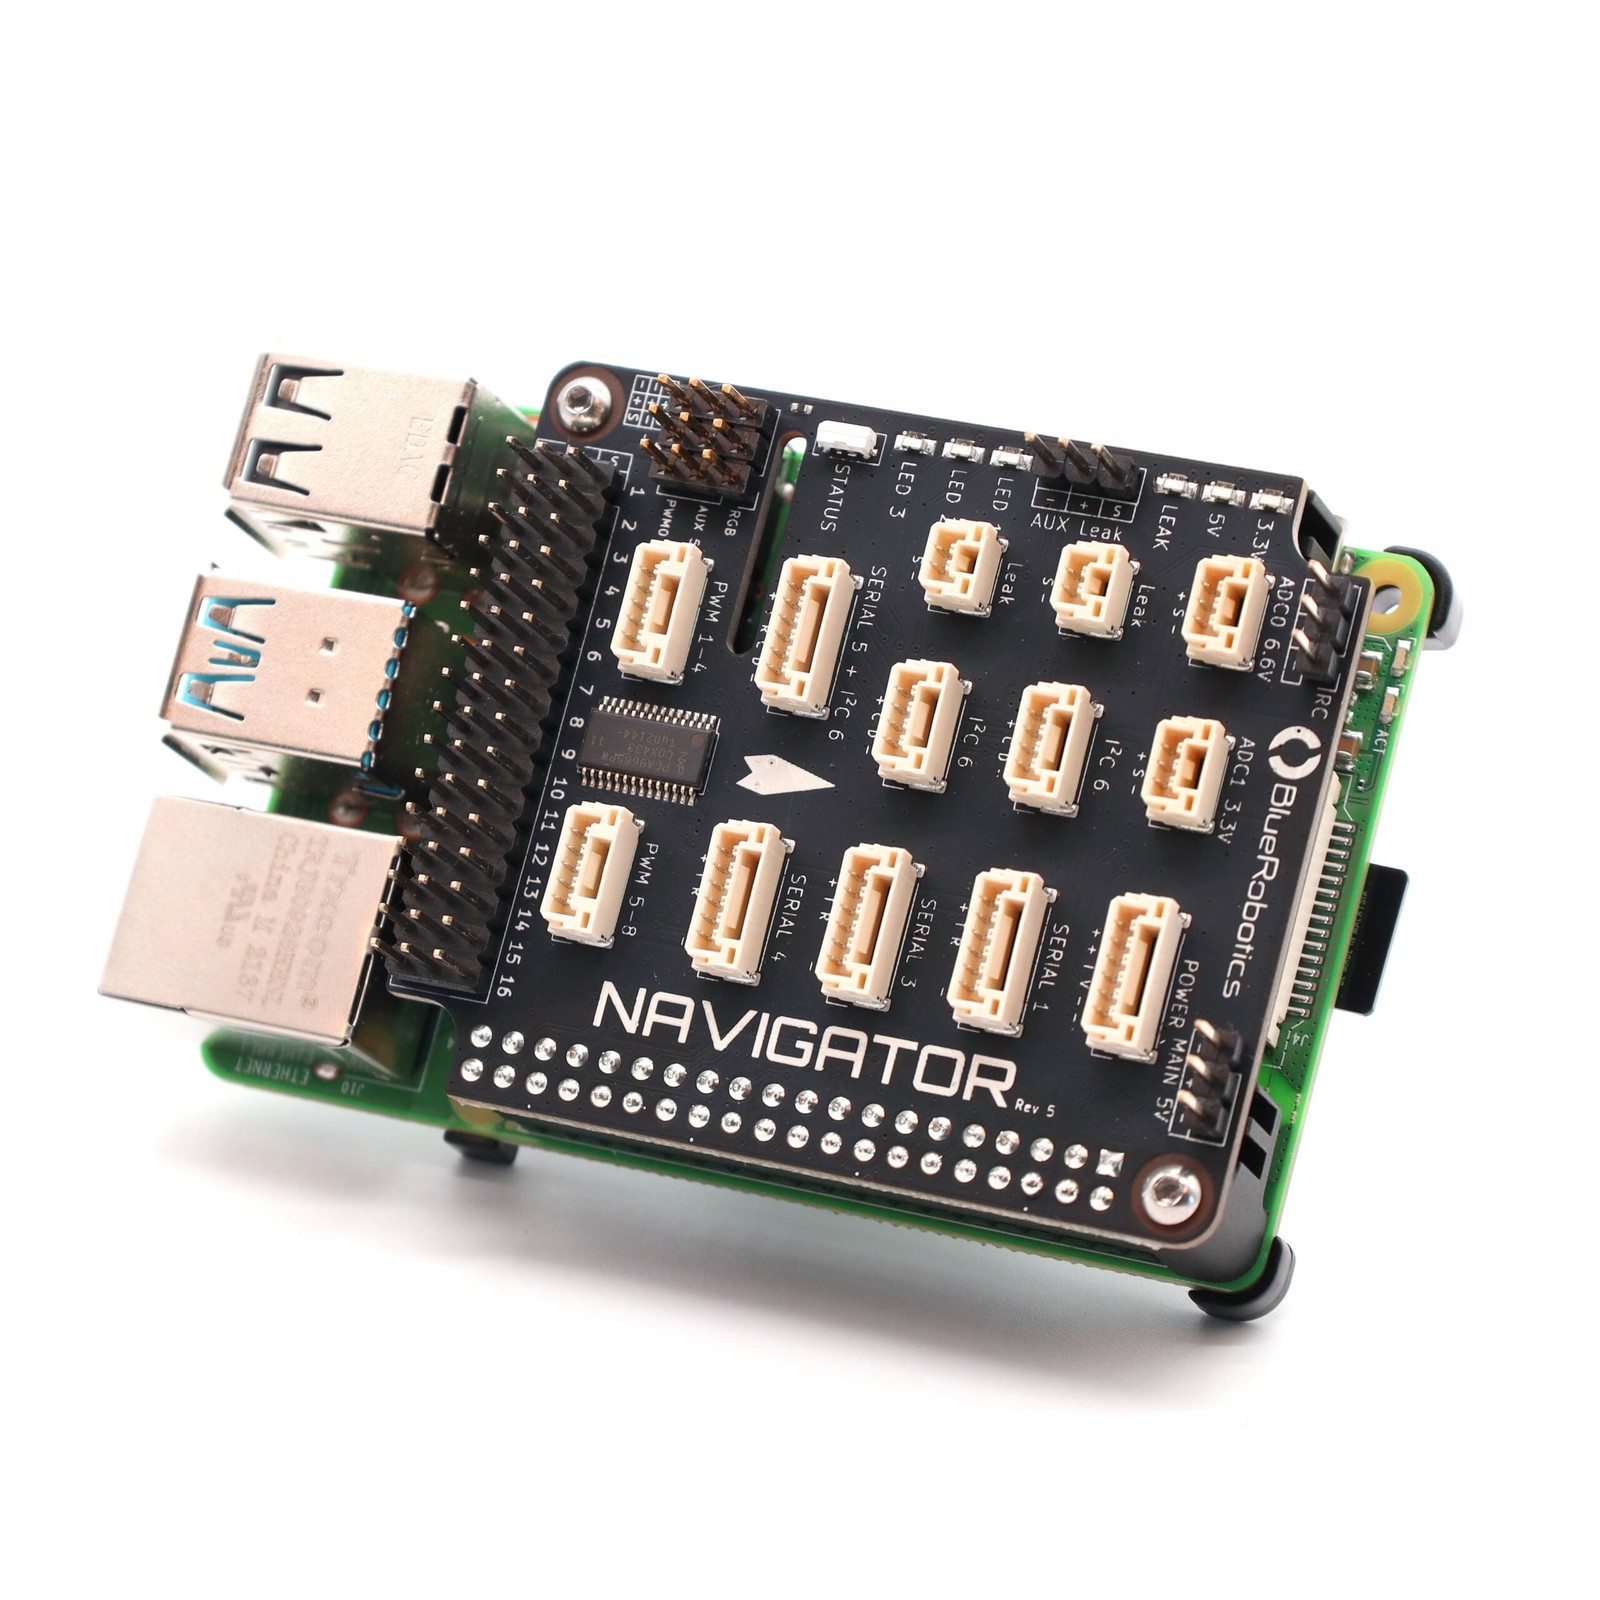
\includegraphics[height=1.25cm, keepaspectratio]{navigator_board.jpg} &
      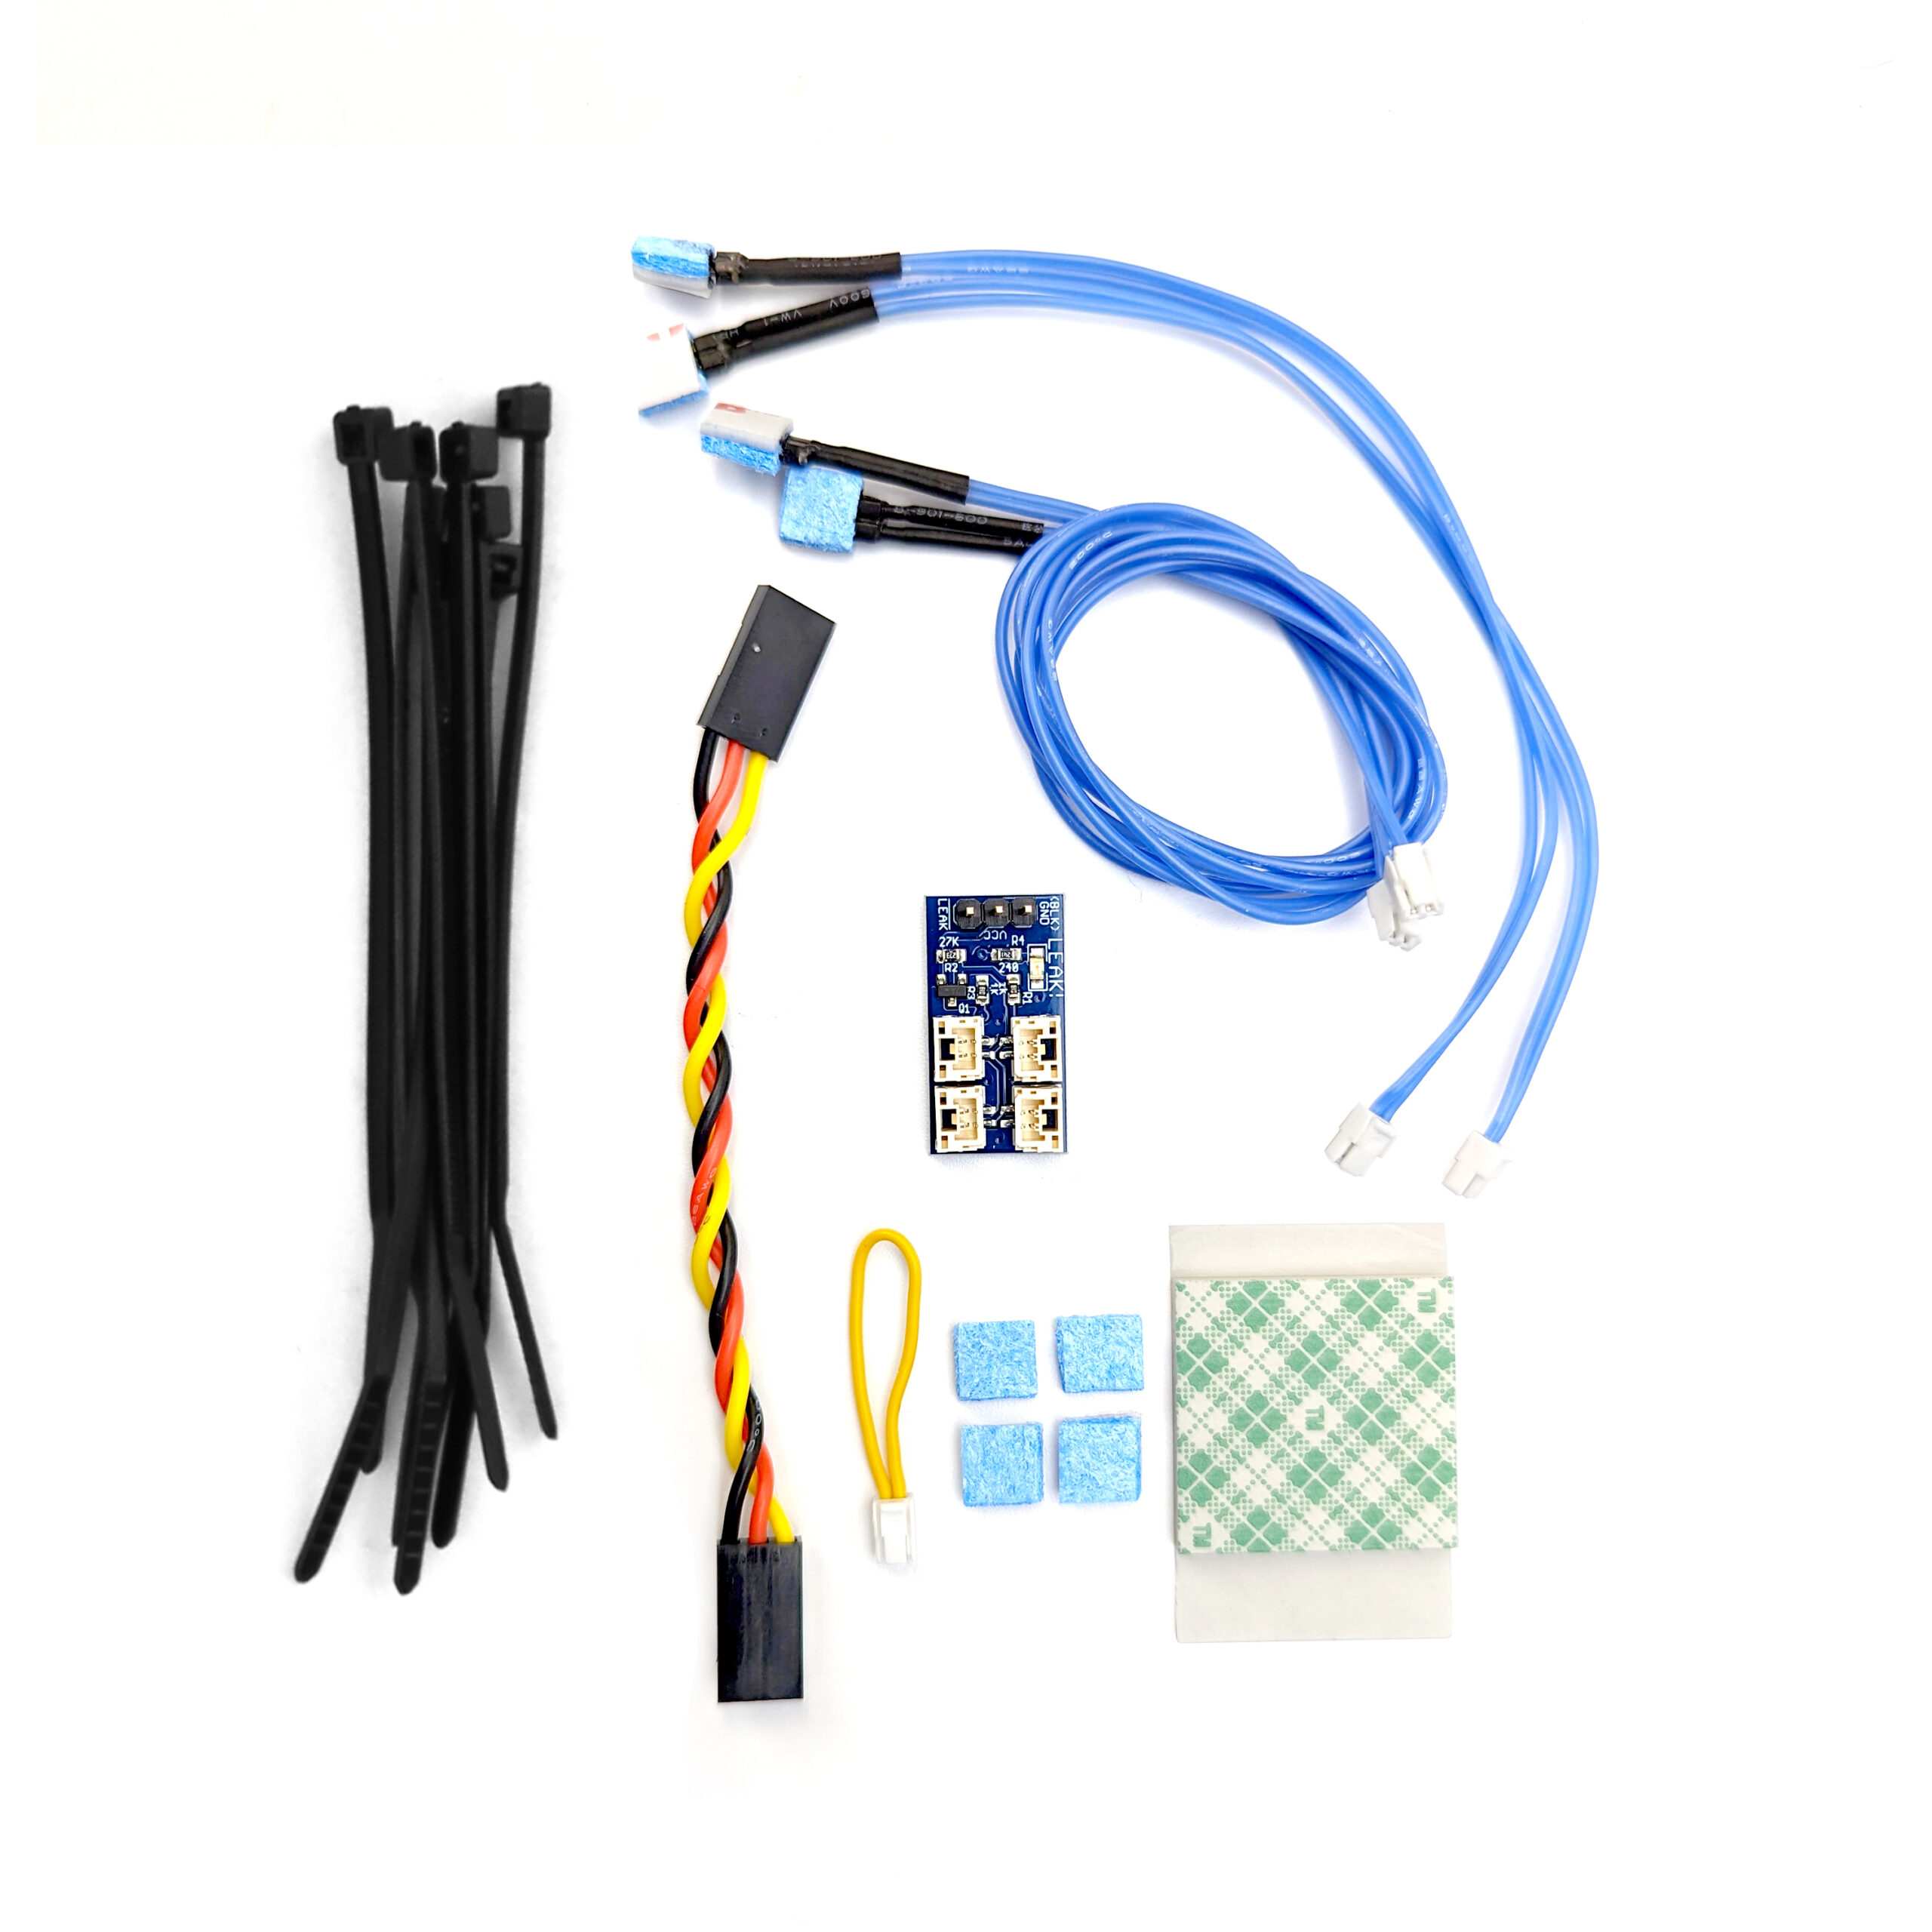
\includegraphics[height=1.25cm, keepaspectratio]{sos_leak_sensor.jpg} &
      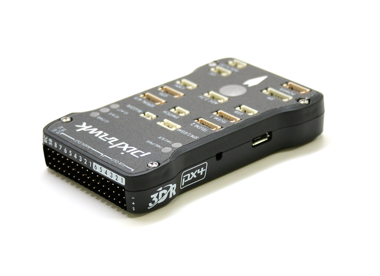
\includegraphics[height=1.25cm, keepaspectratio]{pixhawk_autopilot.png} \\
      \textbf{Raspberry Pi 4} &
      \textbf{Navigator HAT} &
      \textbf{SOS Leak Sensor} &
      \textbf{Pixhawk (Hist.)}
    \end{tabular}%
    }
  \end{center}
  \scriptsize
  \begin{itemize}
    \item \textbf{Tandem Moderne (RPi 4/5 + Navigator)} : carte HAT directe sur GPIO. Double IMU redondante (ICM-20602 + ICM-20948), compas MMC5983MA, 16 PWM, ports JST-GH.
    \item \textbf{Capteurs de Sûreté Véhicule (Vital)} :
      \begin{itemize}\scriptsize
        \item \alertw{SOS Leak Sensors} : rubans conductimétriques au point bas de chaque tube $\rightarrow$ alerte MAVLink instantanée, désarmement propulsion et remontée passive.
        \item \alertw{Capteur Bar02 interne} : monitoring de la dépression post-test de vide $\rightarrow$ détection d'infiltration avant tout contact liquide avec les circuits.
        \item \tech{Power Sense} : monitoring tension/courant Li-ion (prévention décharge/surcharge).
      \end{itemize}
  \end{itemize}
\end{tcolorbox}

\columnbreak

% BLOC 4 : CAISSONS, PENETRATEURS ET CONNECTEURS ETANCHES
\begin{tcolorbox}[title={4. Caissons, Pénétrateurs \& Connecteurs Étanches (Cobalt / SubConn)}]
  \begin{center}
    \resizebox{\linewidth}{!}{%
    \begin{tabular}{cccc}
      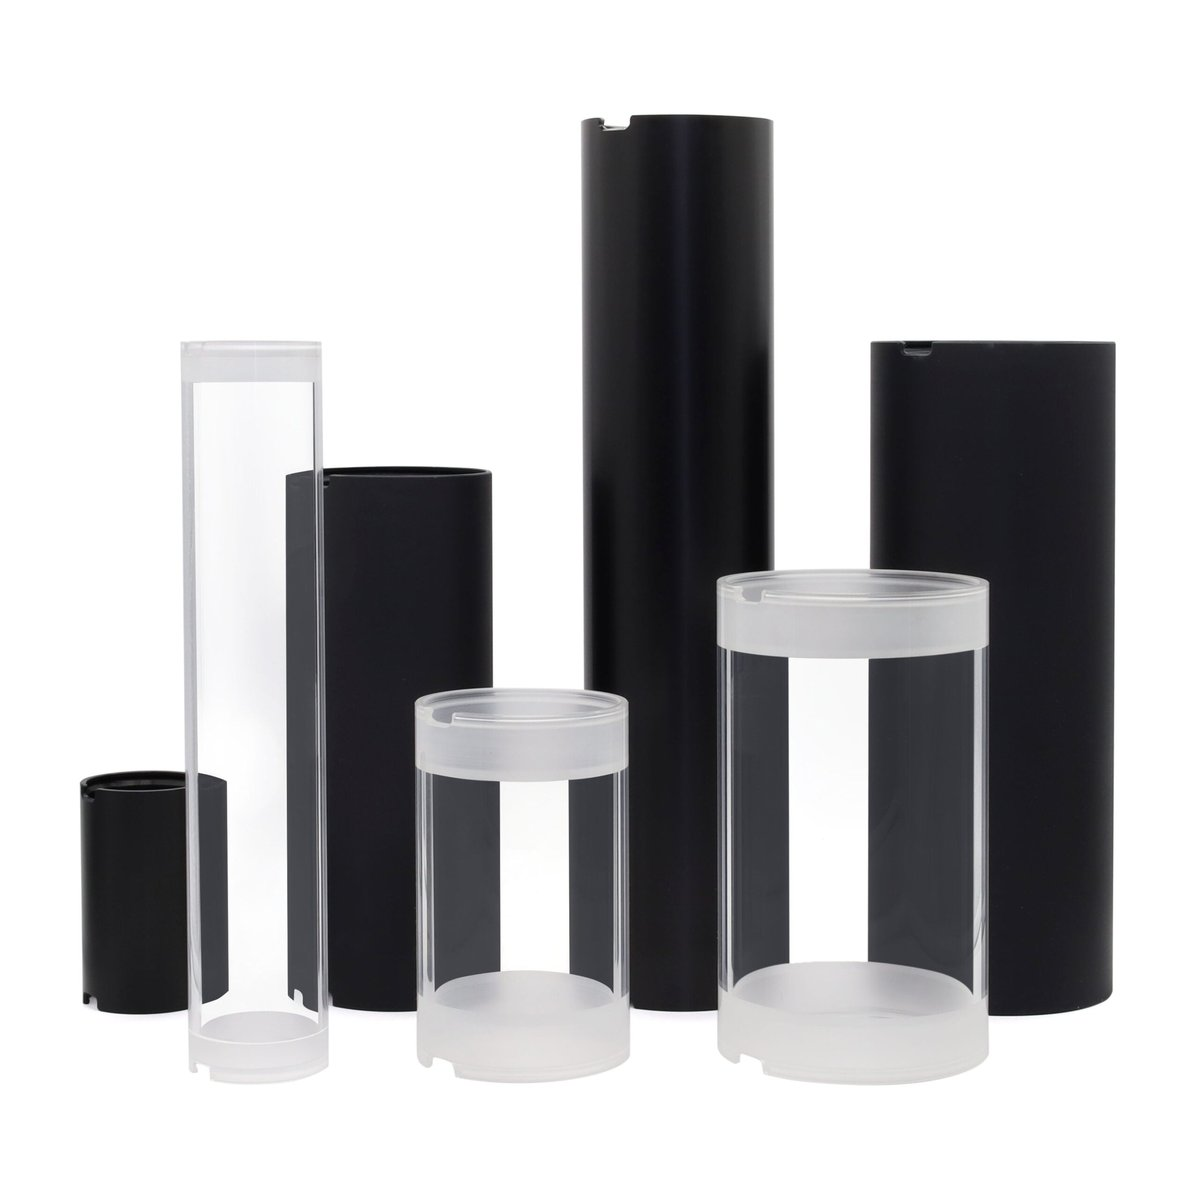
\includegraphics[height=1.15cm, keepaspectratio]{watertight_enclosure.jpg} &
      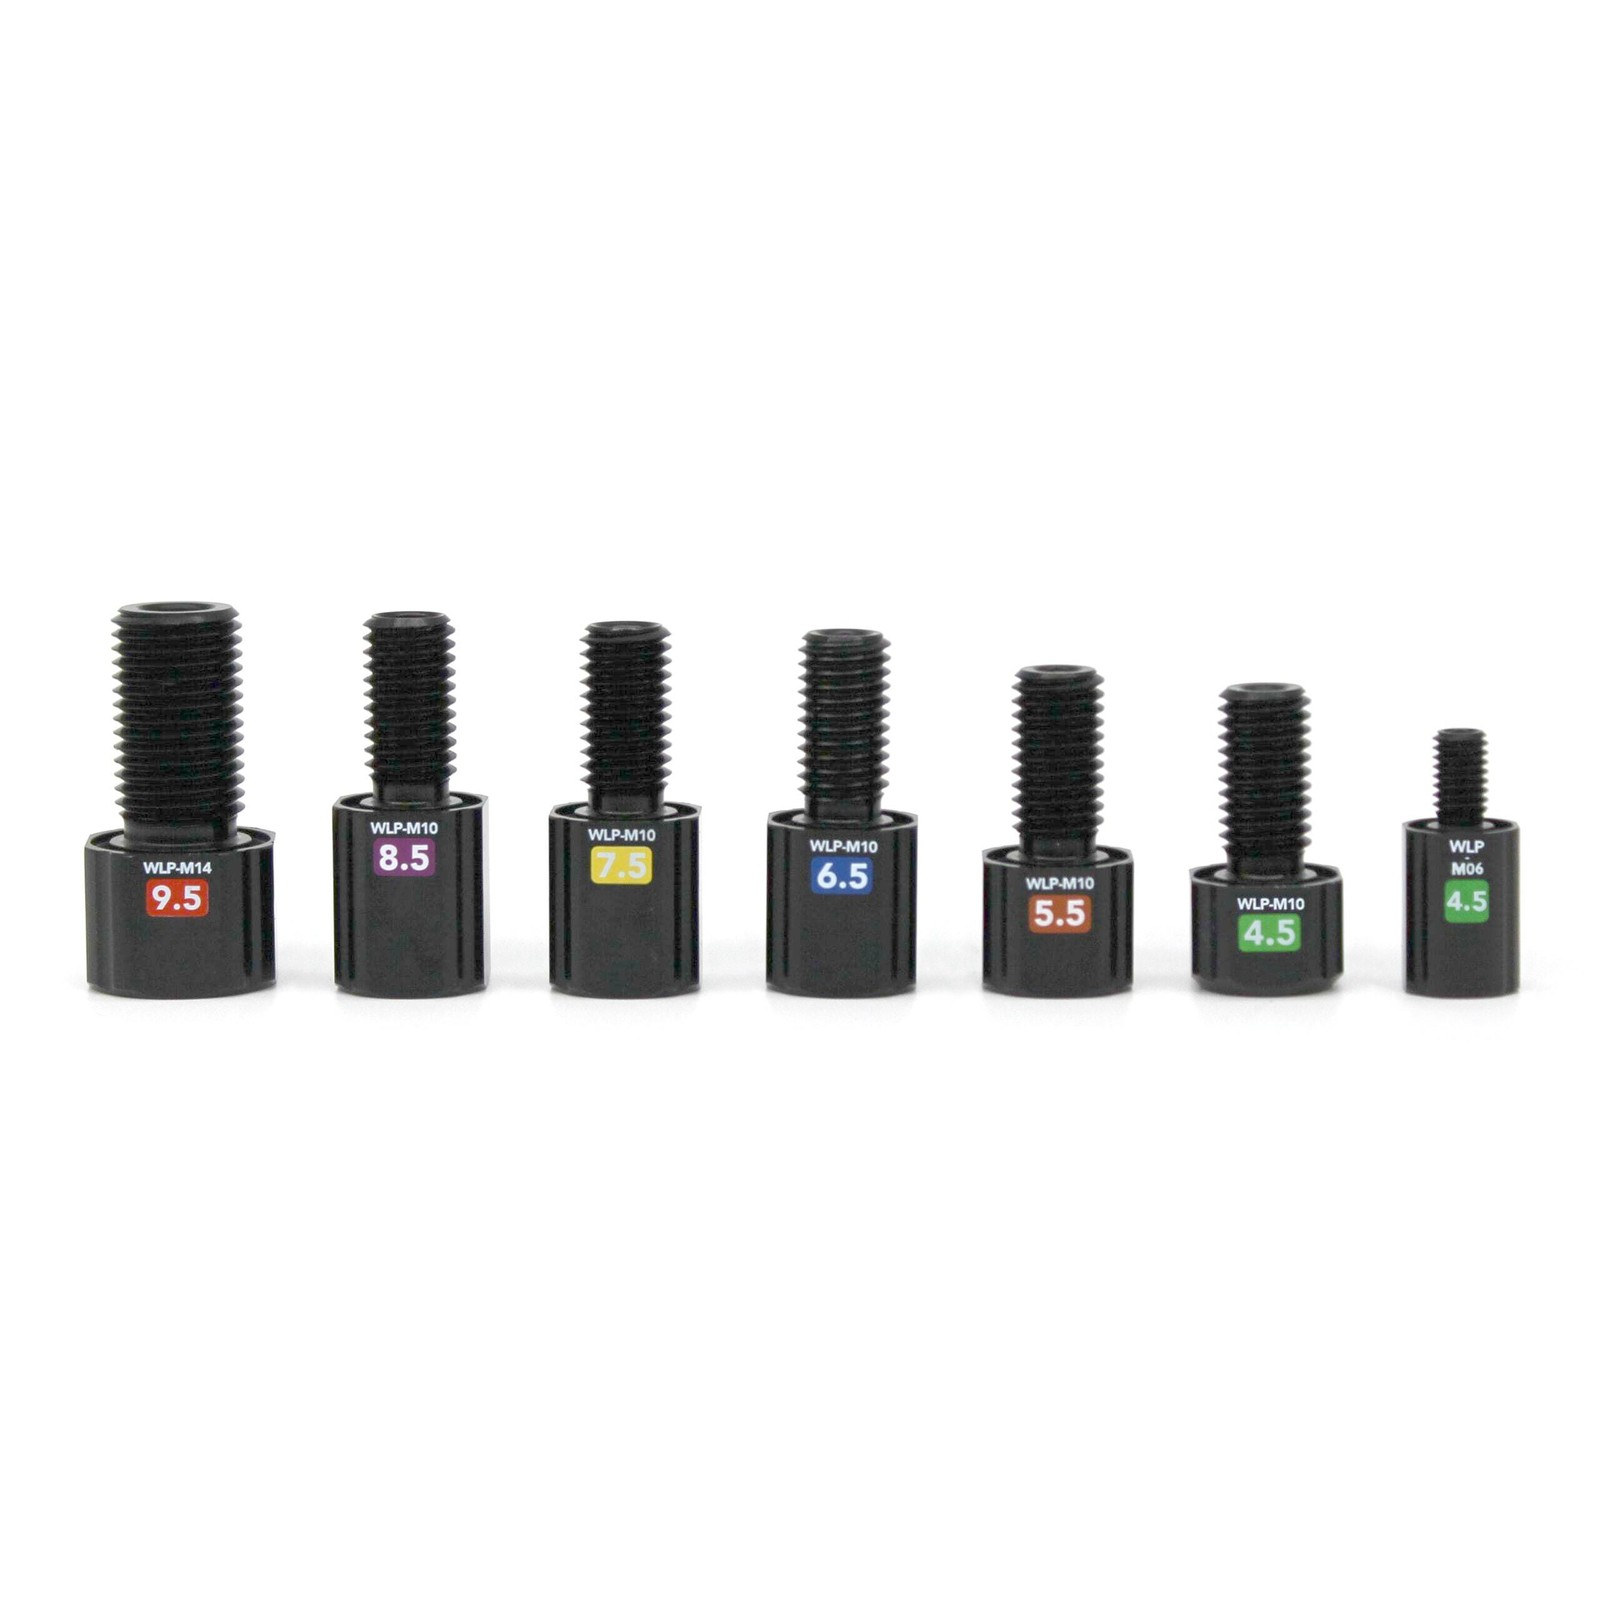
\includegraphics[height=1.15cm, keepaspectratio]{wetlink_penetrator.jpg} &
      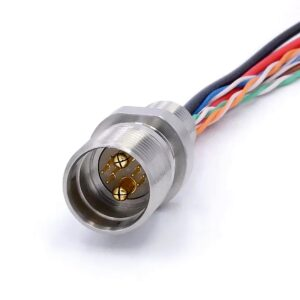
\includegraphics[height=1.15cm, keepaspectratio]{bluetrail_cobalt.jpg} &
      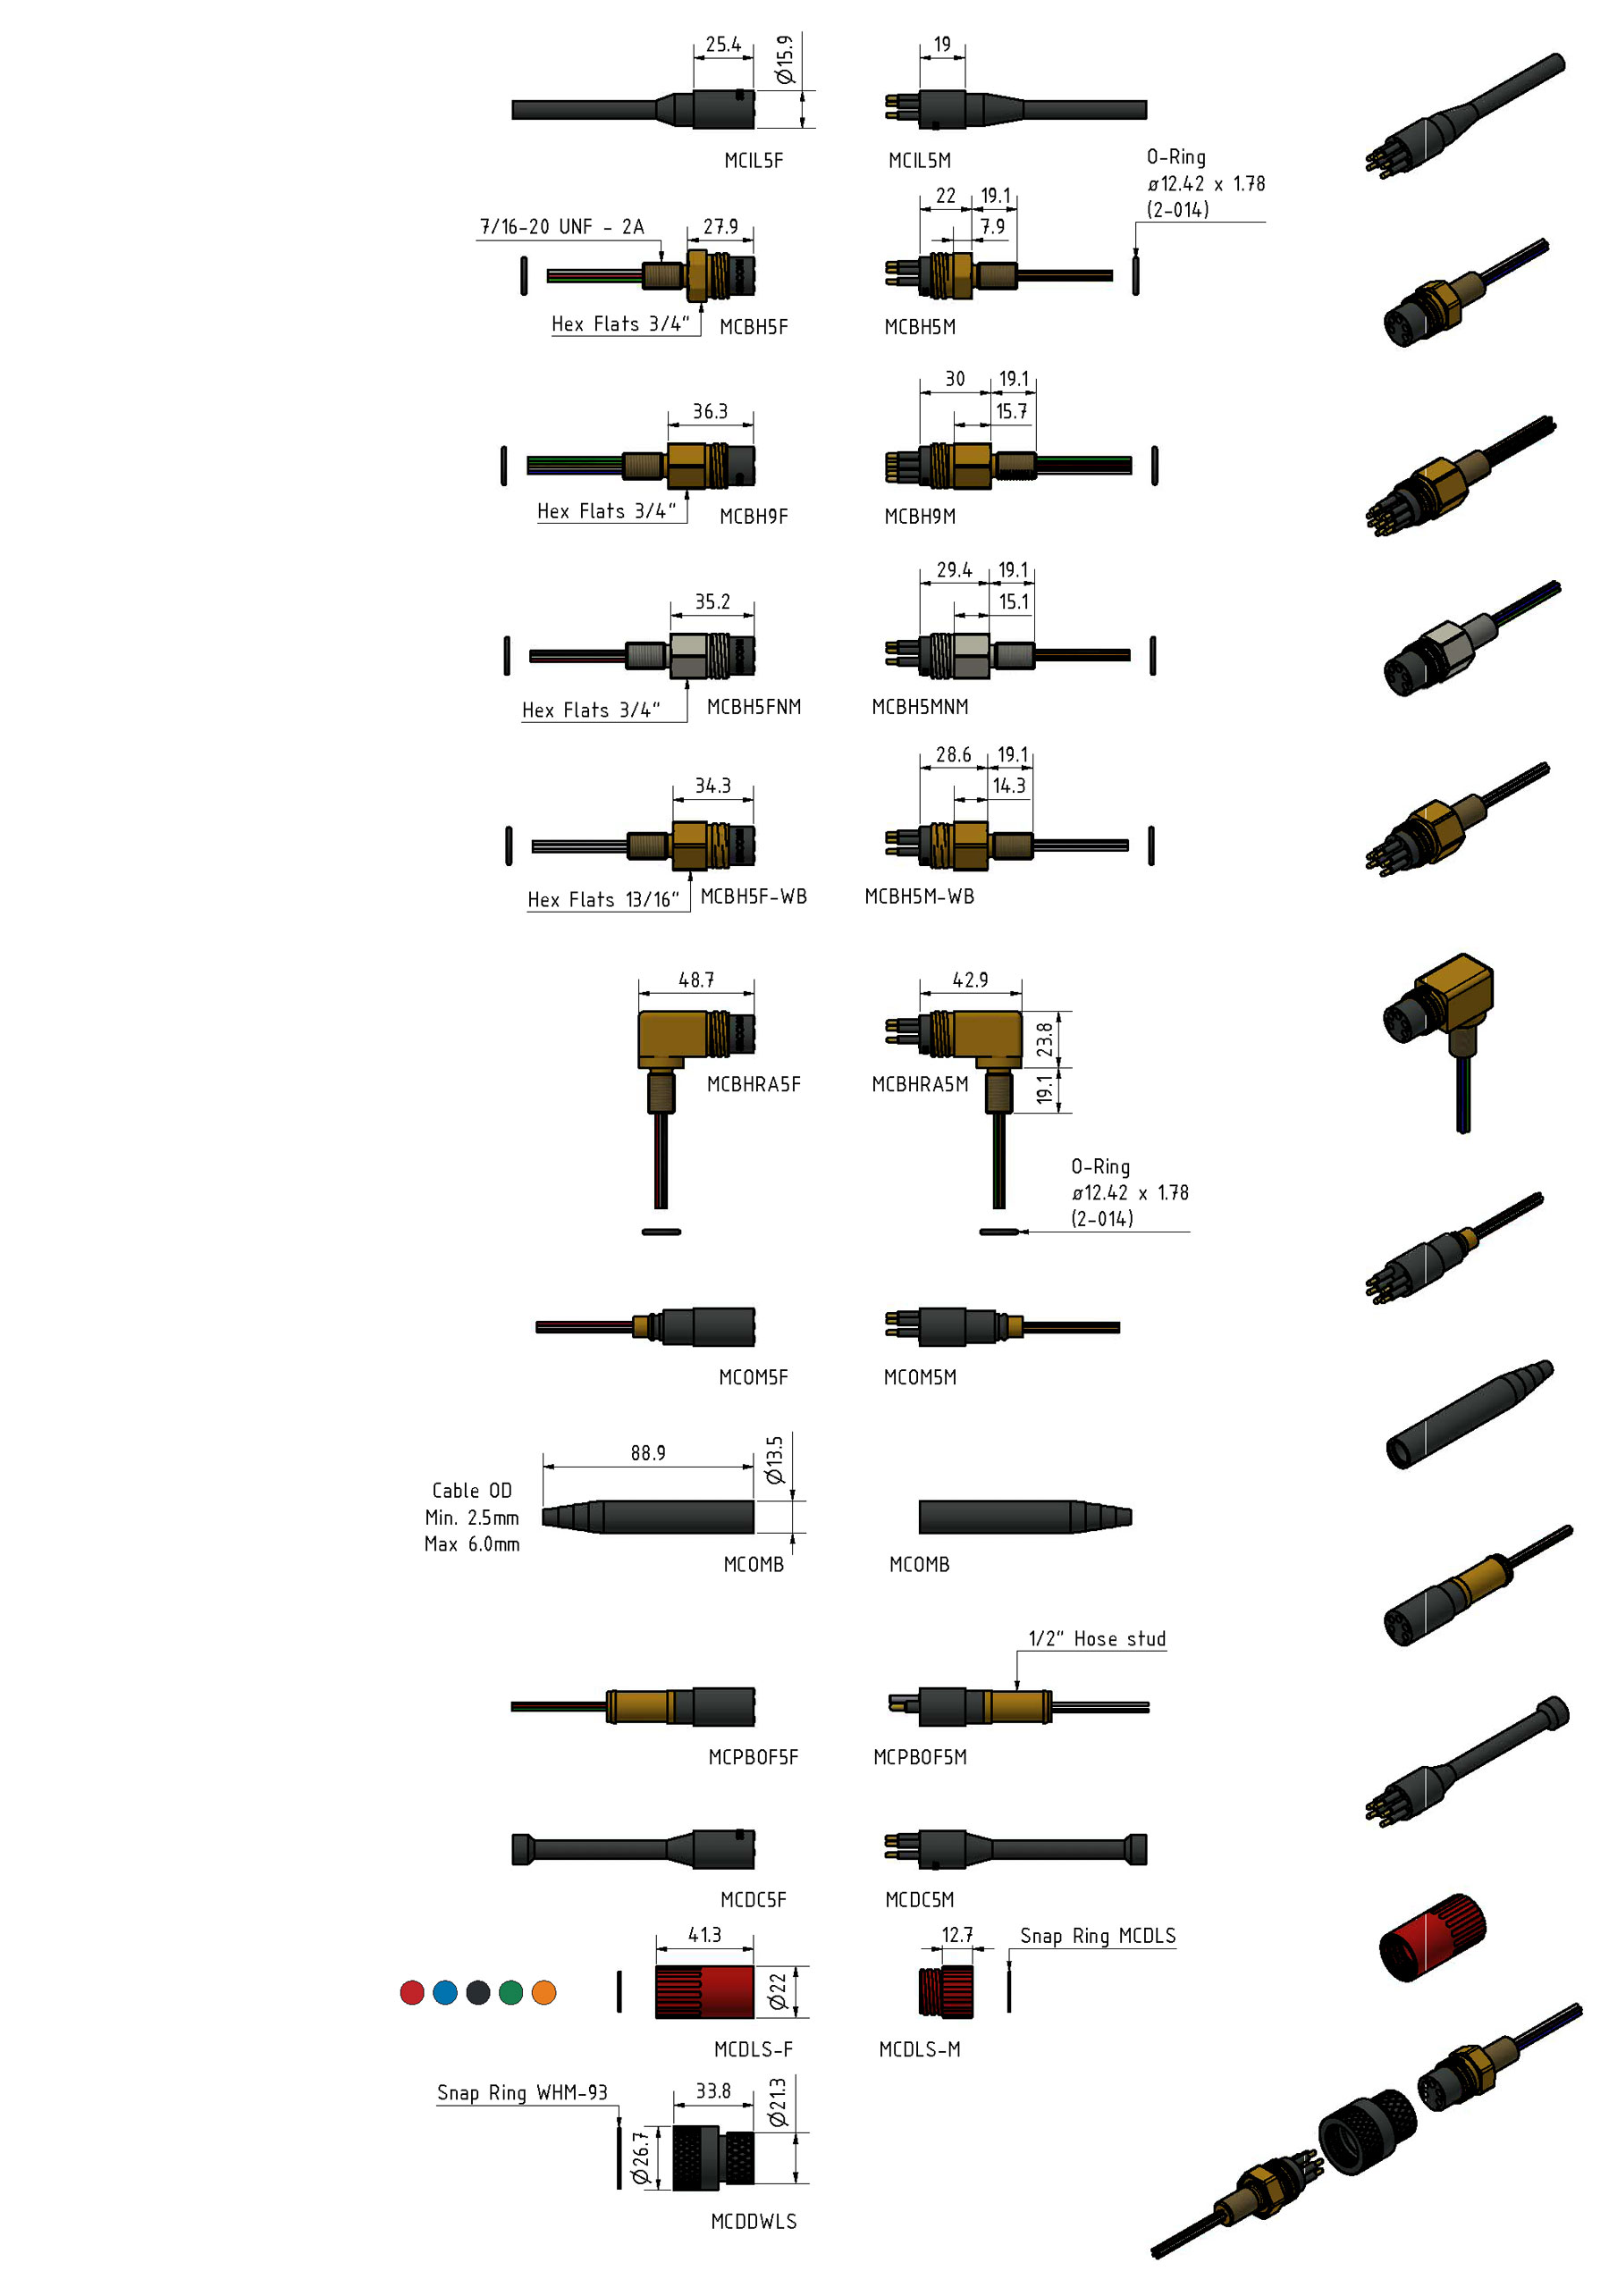
\includegraphics[height=1.15cm, keepaspectratio]{subconn_micro_circular.jpg} \\
      \textbf{Caisson 4"} &
      \textbf{WetLink WLP/JPT} &
      \textbf{Cobalt (Blue Trail)} &
      \textbf{SubConn Micro}
    \end{tabular}%
    }
  \end{center}
  \scriptsize
  \begin{itemize}
    \item \textbf{Caissons 3"/4"} : alu 6061-T6 ($<500\,\text{m}$) ou acrylique ($<150\,\text{m}$), verrouillage cordon flexible (*locking cord*), flasques 14--18 trous M10.
    \item \textbf{Pénétrateurs (WetLink WLP / JPT)} : passage continu étanche ($100\text{--}950\,\text{m}$). Câble captif : changer un composant impose d'ouvrir le caisson.
    \item \textbf{Connecteurs Débrochables} : embase coque + fiche externe. Commande (série, Ethernet) \& puissance ($12\text{--}20\,\text{A}$).
    \item \textbf{Atouts de terrain majeurs} :
      \begin{itemize}\scriptsize
        \item \succw{Remplacement d'un moteur en 2 min} sans ouvrir le caisson (vide intact).
        \item \succw{Ajout de capteurs scientifiques à la volée} (ports aux plug-and-play).
      \end{itemize}
    \item \textbf{Standards} : \textbf{Blue Trail Cobalt} (M10 direct, inox 316/PEEK, $600\,\text{m}$) vs \textbf{SubConn} (standard lourd néoprène Micro Circular).
    \item \textbf{Test de vide obligatoire} : tirer à \succw{$\mathbf{-0.5\,\text{bar}}$} pendant 15 min avant mise à l'eau.
  \end{itemize}
\end{tcolorbox}

% BLOC 5 : ENERGIE EMBARQUEE ET CHUTE DE TENSION
\begin{tcolorbox}[title={5. Énergie Embarquée : Pourquoi Enfermer la Batterie ?}]
  \begin{center}
    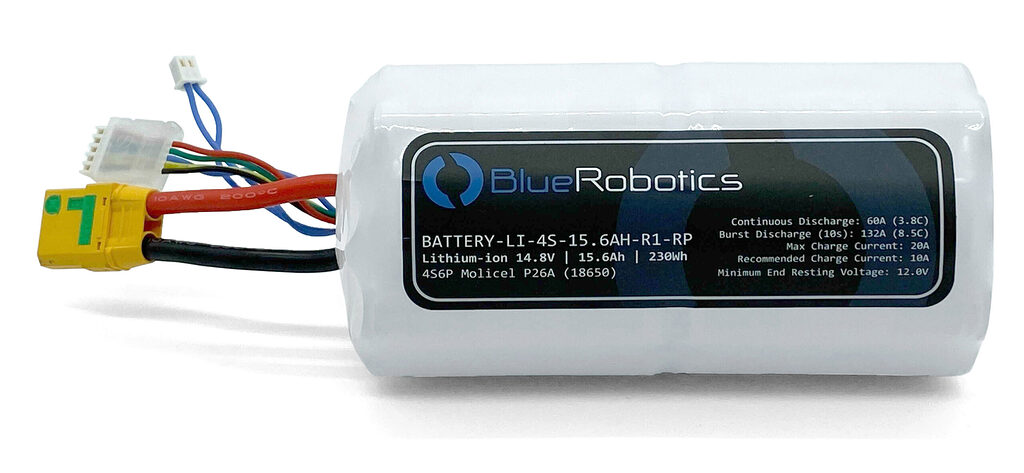
\includegraphics[height=1.2cm, keepaspectratio]{battery_pack.jpg}\\
    \tiny\textbf{Pack Batterie Li-ion 4S ($14.8\,\text{V}$, $18\,\text{Ah}$ / $266\,\text{Wh}$) logé en caisson 3" bas}
  \end{center}
  \scriptsize
  \begin{itemize}
    \item \textbf{Stabilité passive} : masse lourde ($1.2\,\text{kg}$) au fond pour garantir le centre de carène $B$ au-dessus de $G$ ($C = m g \overline{BG} \sin\theta$).
    \item \textbf{Physique de la chute de tension} : un ROV consomme $I = \mathbf{30\text{--}60\,\text{A}}$. Sur un ombilical fin de 100--300m ($R \approx 2\,\Omega$) :
      \[
        \Delta V = R \cdot I = 2\,\Omega \times 30\,\text{A} = \mathbf{60\,\text{V}} \quad (\gg 14.8\,\text{V} !)
      \]
      Une alimentation 14.8V depuis la surface s'écroulerait instantanément à 0V !
    \item \textbf{Pertes Joule colossales} : $P = R \cdot I^2 = 2 \times 30^2 = \mathbf{1800\,\text{W}}$ dissipés en chaleur (fusion du câble). L'énergie \alertw{doit être enfermée dans le robot} ou transmise en haute tension (OTPS 400V).
  \end{itemize}
\end{tcolorbox}

% BLOC 6 : CHECKLIST PRE-PLONGEE
\begin{tcolorbox}[title={6. Checklist Opérationnelle Avant la Mise à l'Eau}]
  \scriptsize
  \begin{enumerate}
    \item \textbf{Veille PING \& Légalité} : consulter PING (\href{https://portail.ping-info-nautique.fr/}{\underline{portail.ping-info-nautique.fr}}) et vérifier la présence d'un Capitaine 200 (si ASV/AUV en mer).
    \item Inspecter les joints toriques sous loupe (zéro grain de sable, graissage très fin).
    \item Contrôler le serrage des écrous WetLink / JPT et bagues de connecteurs Cobalt / SubConn.
    \item Valider le test de vide terrain ($-0.5\,\text{bar}$ pendant 15 minutes).
    \item Vérifier la flottabilité positive nette (+200 à +500 g) et tension Li-ion ($>16\,\text{V}$).
  \end{enumerate}
\end{tcolorbox}

\end{multicols}

\vspace{-6pt}
\begin{center}
  \scriptsize\textcolor{gray}{Mémento ANF ArchiDrone 2026 --- Réseaux Drone\&Cap' \& 2RM (Réseau Métier Roboticien et Mécatronicien) --- Page 1 : Matériel \& Mécatronique (Tournez la page pour l'Acoustique, Essais \& Données)}
\end{center}

\newpage

% ==============================================================================
% PAGE 2 : CAPTEURS, ACOUSTIQUE, ARCHITECTURE ESSAIS & ALIM HAUTE TENSION (VERSO)
% ==============================================================================
\begin{center}
  {\small\bfseries\textcolor{OceanDeep}{ANF ArchiDrone 2026 --- Réseaux Drone\&Cap' \& 2RM (Réseau Métier Roboticien et Mécatronicien)}} \\
  \vspace{1pt}
  {\large\bfseries\textcolor{OceanMedium}{Mémento Technique : Capteurs, Acoustique, Essais \& Énergie OTPS}} \\
  \vspace{1pt}
  {\scriptsize\textit{Formateur : Quentin Brateau --- 04 Novembre 2026 --- Caméras, feux Lumen, Bar30/02, sonars, DVL, Station Sol, FXTI, RC \& OTPS 400V}}
\end{center}
\vspace{-9pt}
\hrule height 0.8pt
\vspace{2pt}

\begin{multicols}{2}

% BLOC 7 : VISION, LUMIERES ET CAPTEURS DE PRESSION
\begin{tcolorbox}[title={7. Recueil de Données : Caméras HD/4K, Lumières Lumen \& Bar30}]
  \begin{center}
    \resizebox{\linewidth}{!}{%
    \begin{tabular}{cccc}
      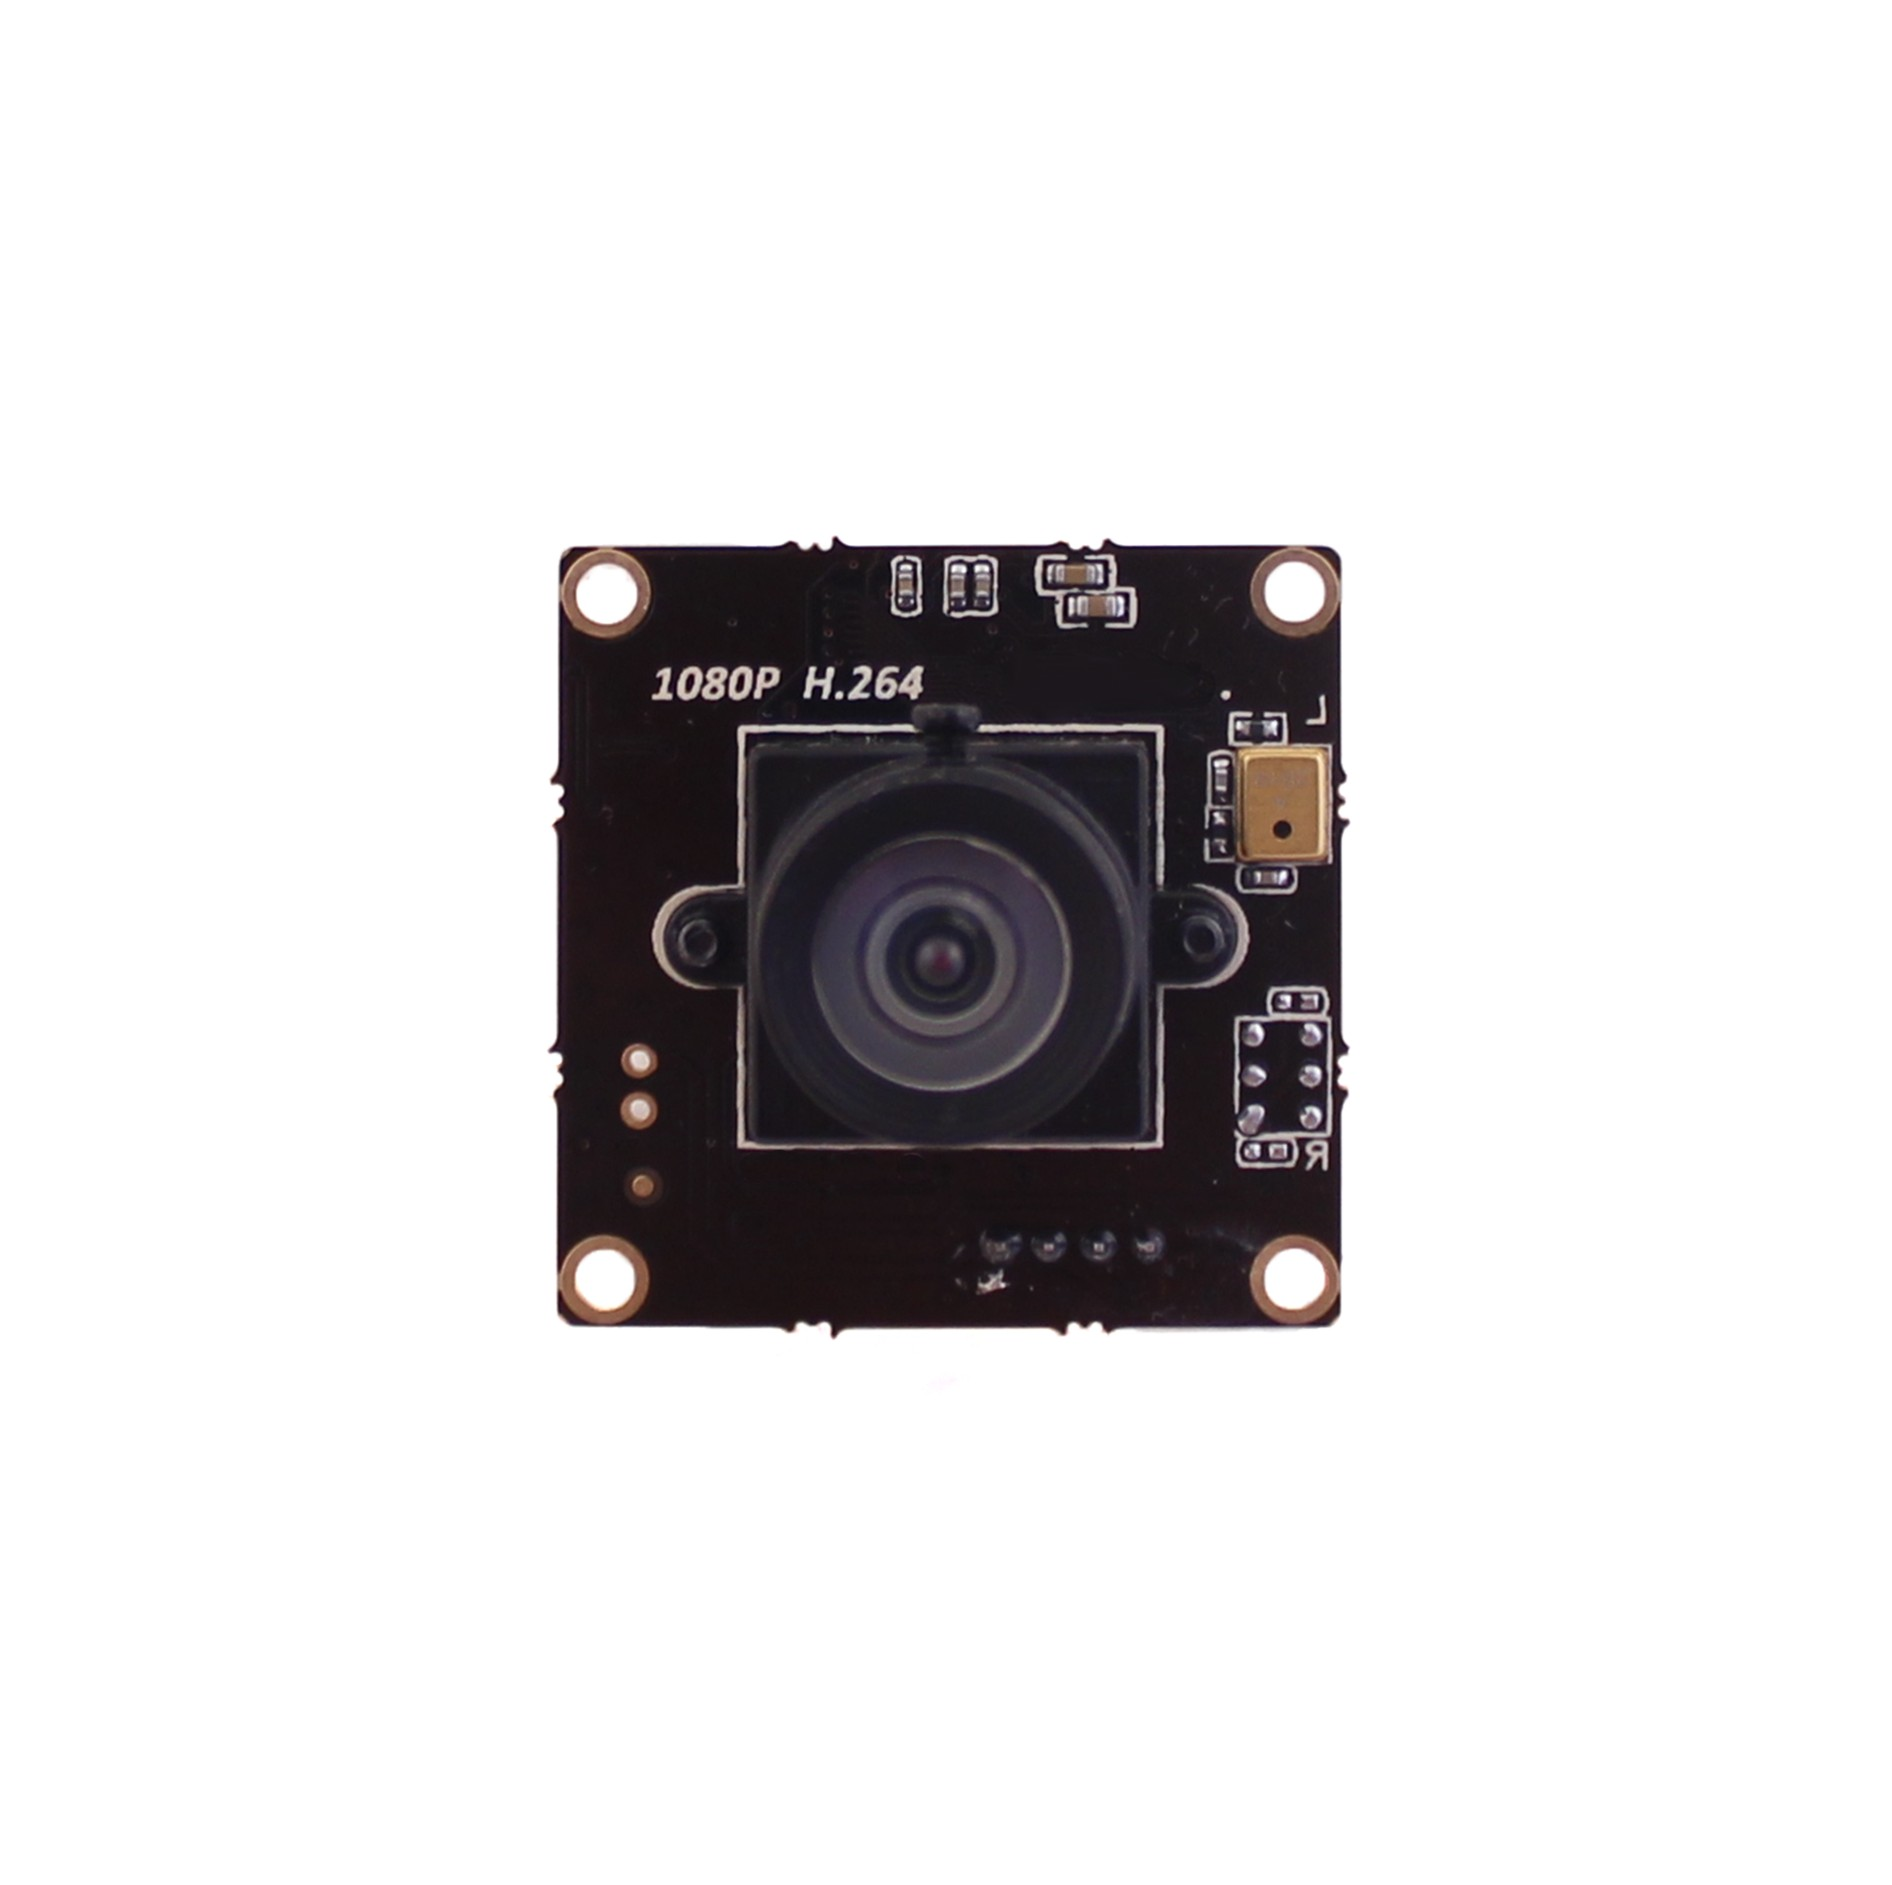
\includegraphics[height=1.20cm, keepaspectratio]{camera_hd.jpg} &
      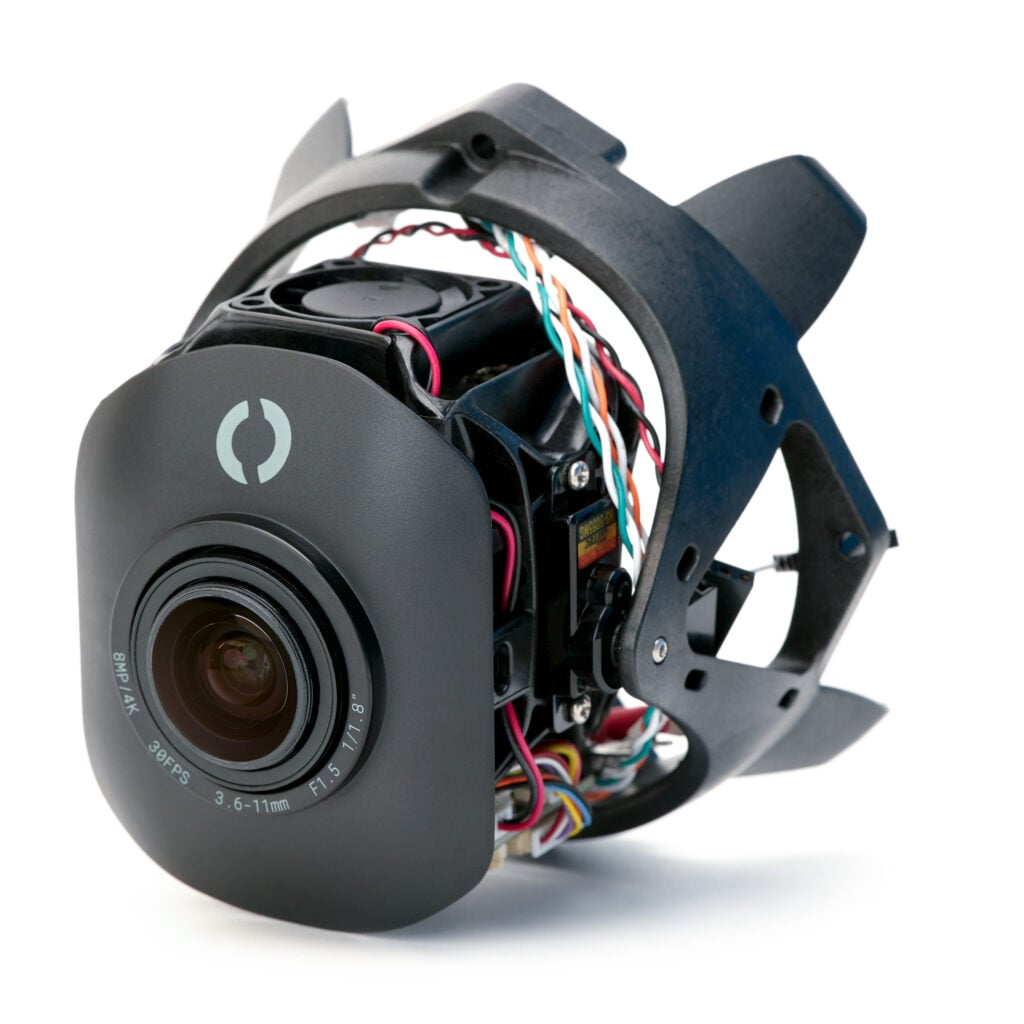
\includegraphics[height=1.20cm, keepaspectratio]{camera_4k.jpg} &
      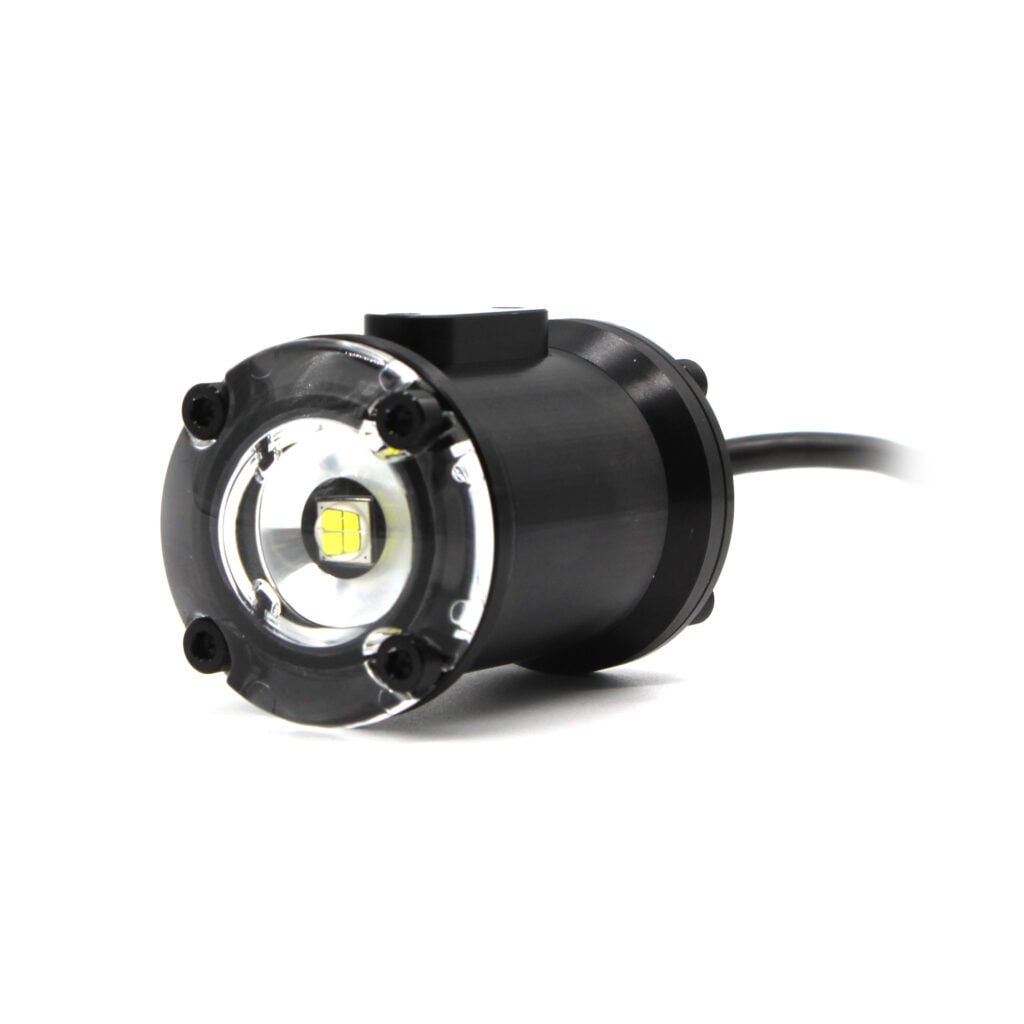
\includegraphics[height=1.20cm, keepaspectratio]{lumen_light.jpg} &
      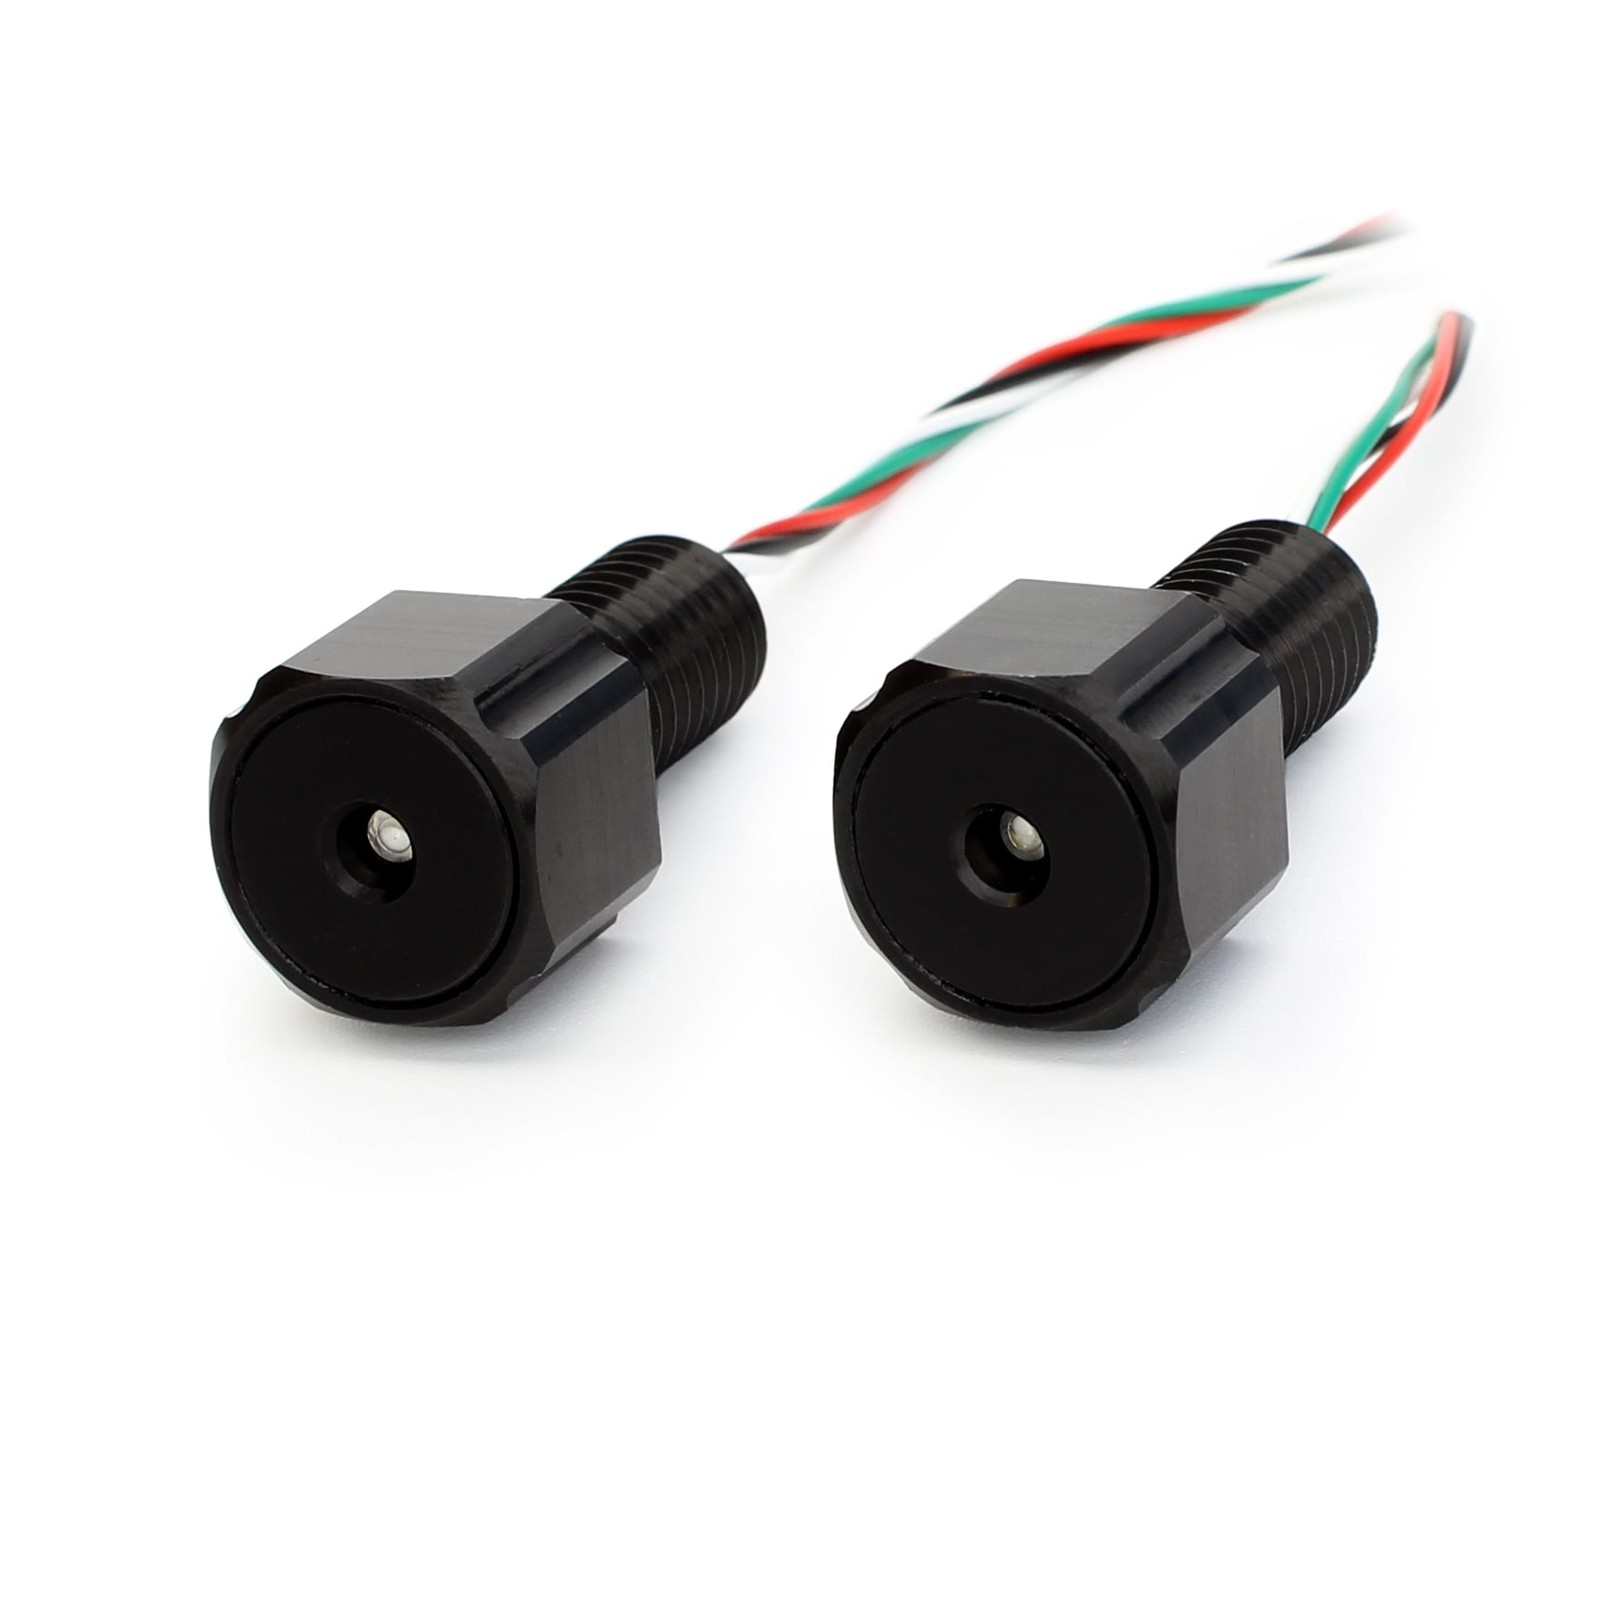
\includegraphics[height=1.20cm, keepaspectratio]{bar30_sensor.jpg} \\
      \textbf{Caméra Low-Light HD} &
      \textbf{Nouvelle 4K Cam} &
      \textbf{Lumière Lumen} &
      \textbf{Pression Bar30}
    \end{tabular}%
    }
  \end{center}
  \scriptsize
  \begin{itemize}
    \item \textbf{Bar30 (MS5837-30BA)} : résolution \succw{$\mathbf{0.2\,\text{mm}}$ d'eau}, bus I2C (\code{0x76}). Asservissement en profondeur (*Depth Hold*) et altitude sous ArduSub.
    \item \textbf{Bar02 (MS5837-02BA)} : ultra-haute résolution ($<0.05\,\text{mm}$) pour lacs, marégraphie et surveillance de dépression interne.
    \item \textbf{Caméras Étanches Low-Light HD} : capteur haute sensibilité, dôme acrylique, nacelle tilt motorisée ($0^\circ$ à $-90^\circ$ benthique), photogrammétrie 3D.
    \item \textbf{Lumières Étanches Lumen ($1500\text{--}6000\,\text{lm}$)} : restaurent le spectre rouge absorbé sous l'eau. Montage déporté éliminant la rétrodiffusion (*backscatter*).
    \item \textbf{Lasers de Dimension} : pointeurs parallèles distants de $50\text{--}100\,\text{mm}$ pour échelle métrique sans contact sur la faune et le benthos.
  \end{itemize}
\end{tcolorbox}

% BLOC 8 : SONARS & MBES
\begin{tcolorbox}[title={8. Acoustique Sous-Marine : Sonars, Omniscan \& MBES}]
  \begin{center}
    \resizebox{\linewidth}{!}{%
    \begin{tabular}{cc}
      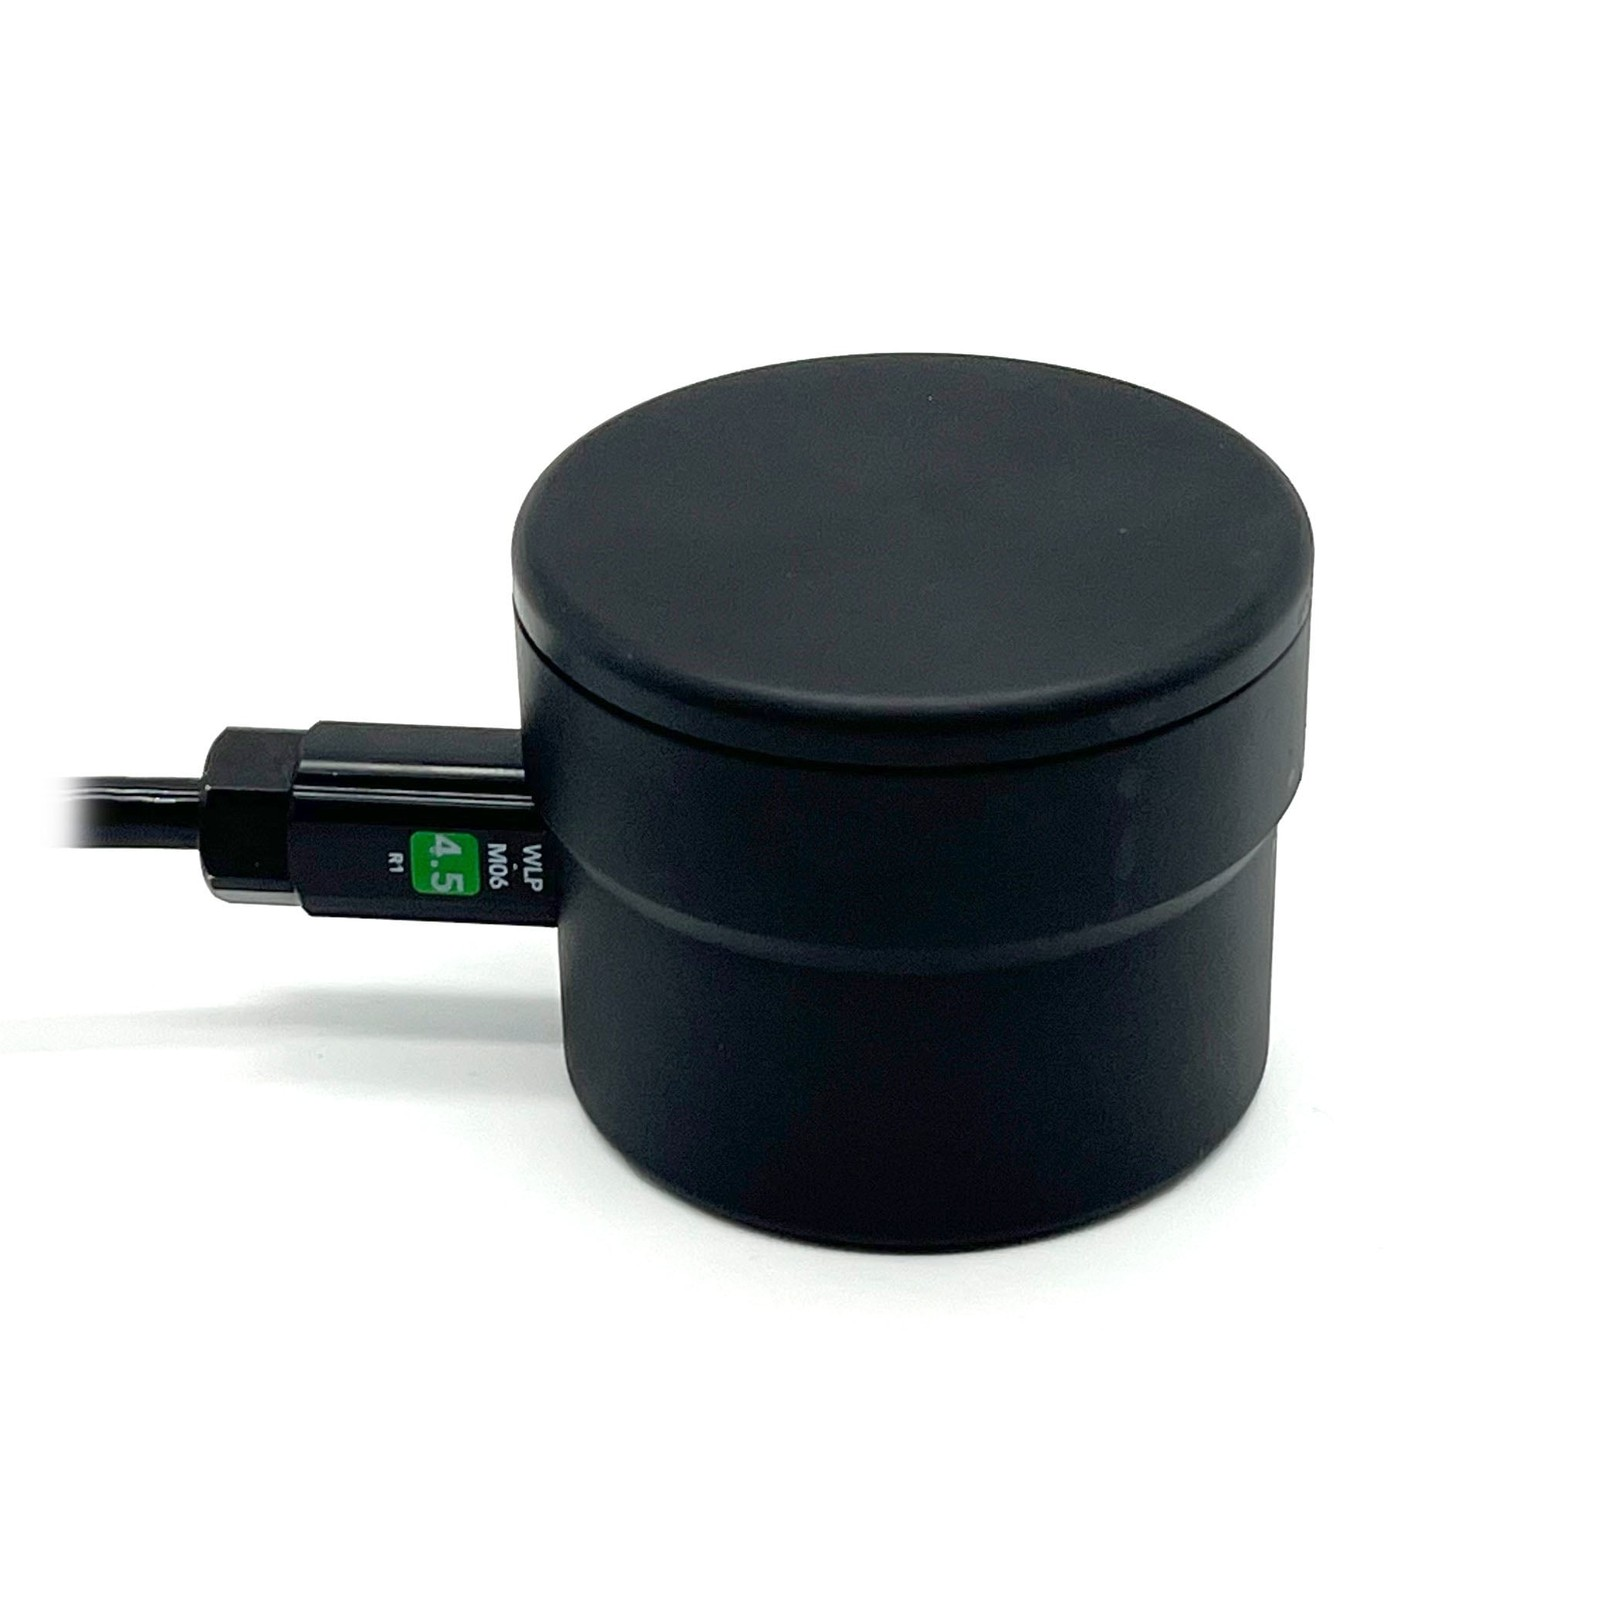
\includegraphics[height=1.25cm, keepaspectratio]{ping_echosounder.jpg} &
      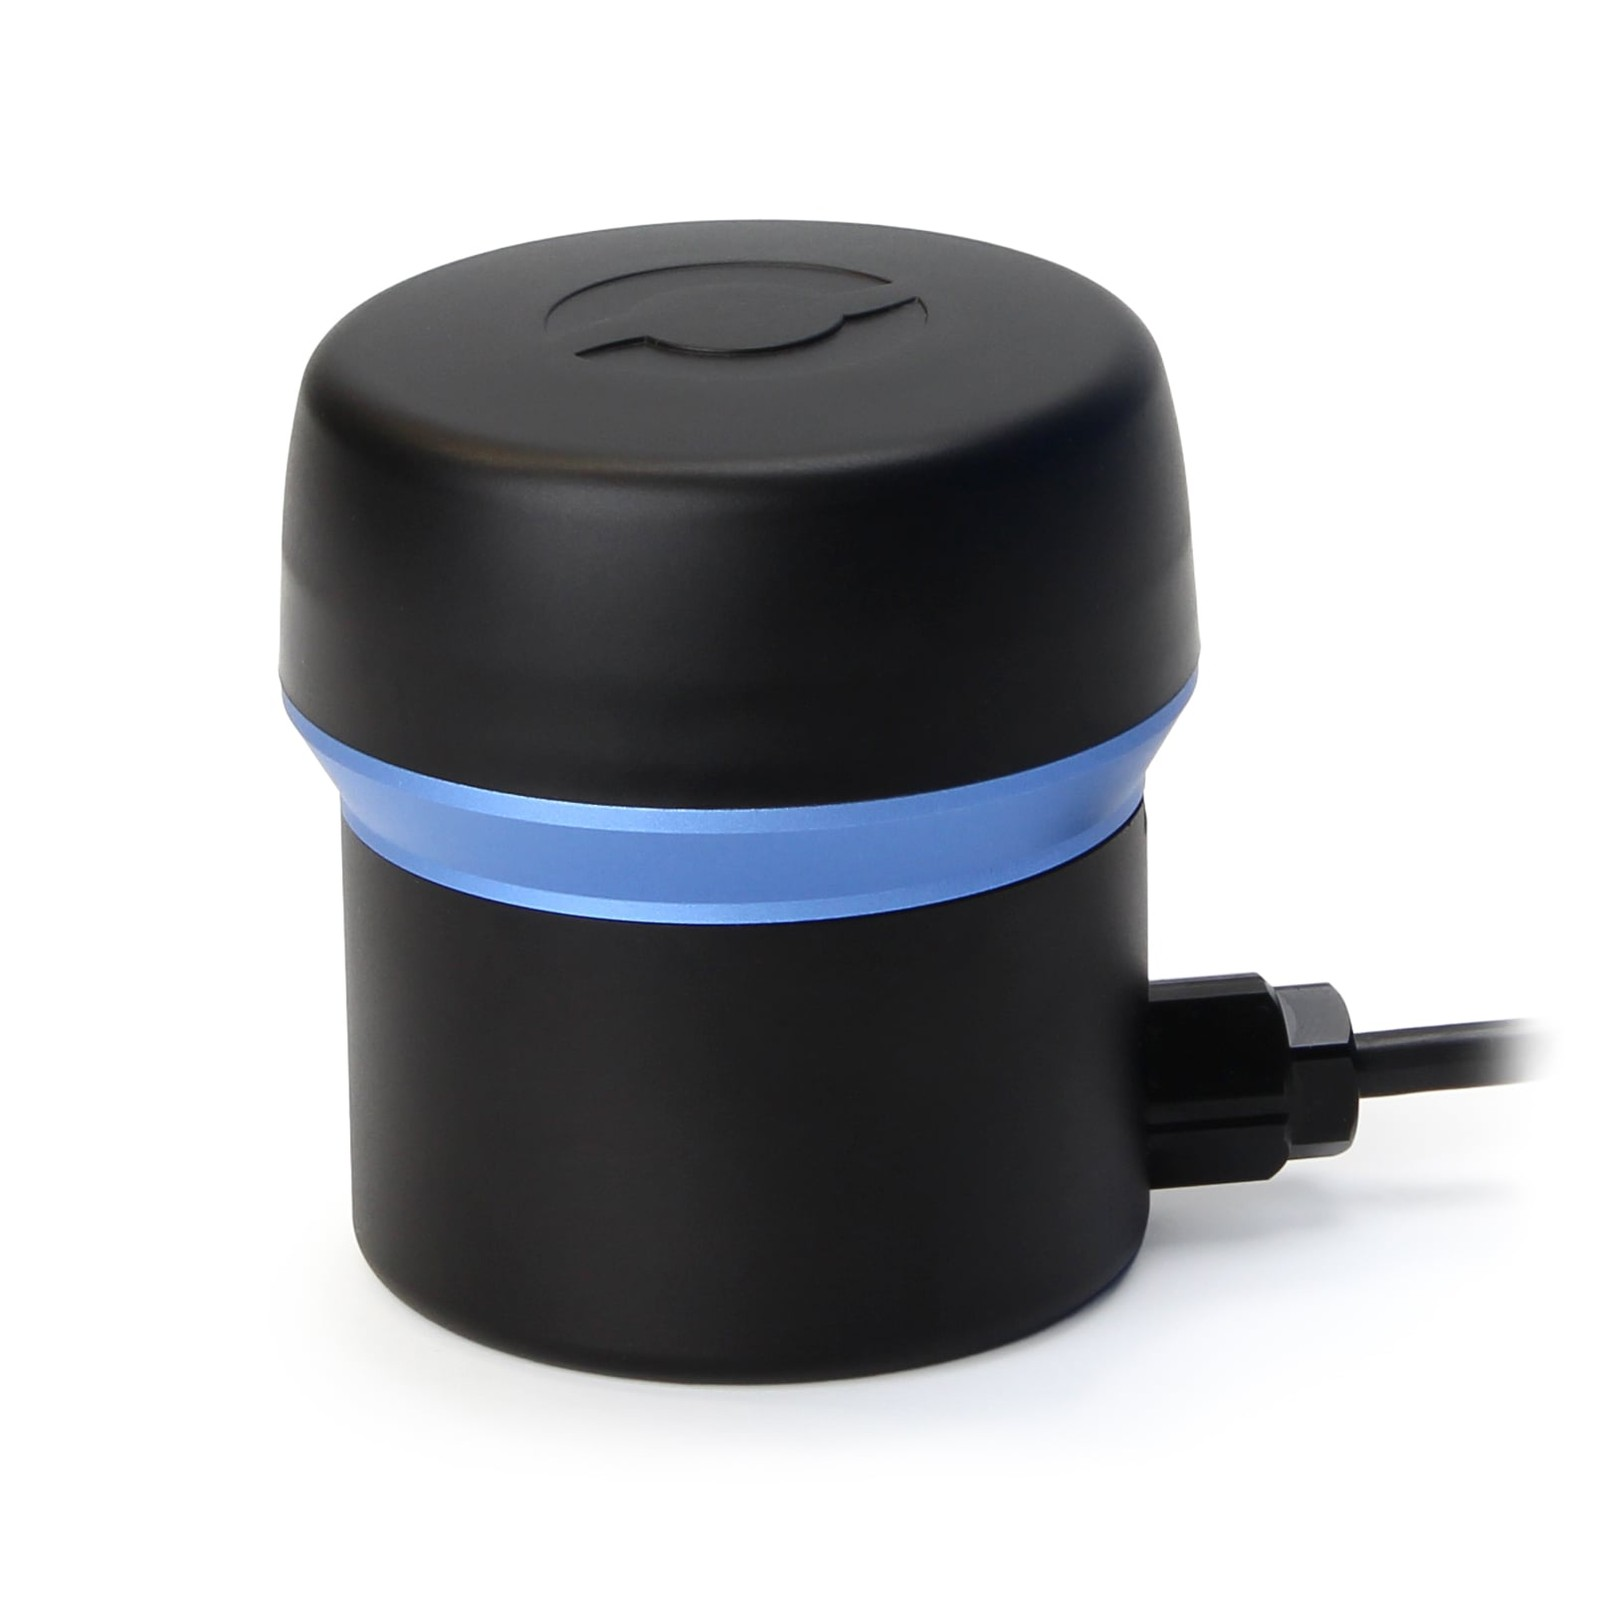
\includegraphics[height=1.25cm, keepaspectratio]{ping360_sonar.jpg} \\
      \textbf{Ping Sonar (115 kHz)} &
      \textbf{Ping360 (750 kHz)} \\
      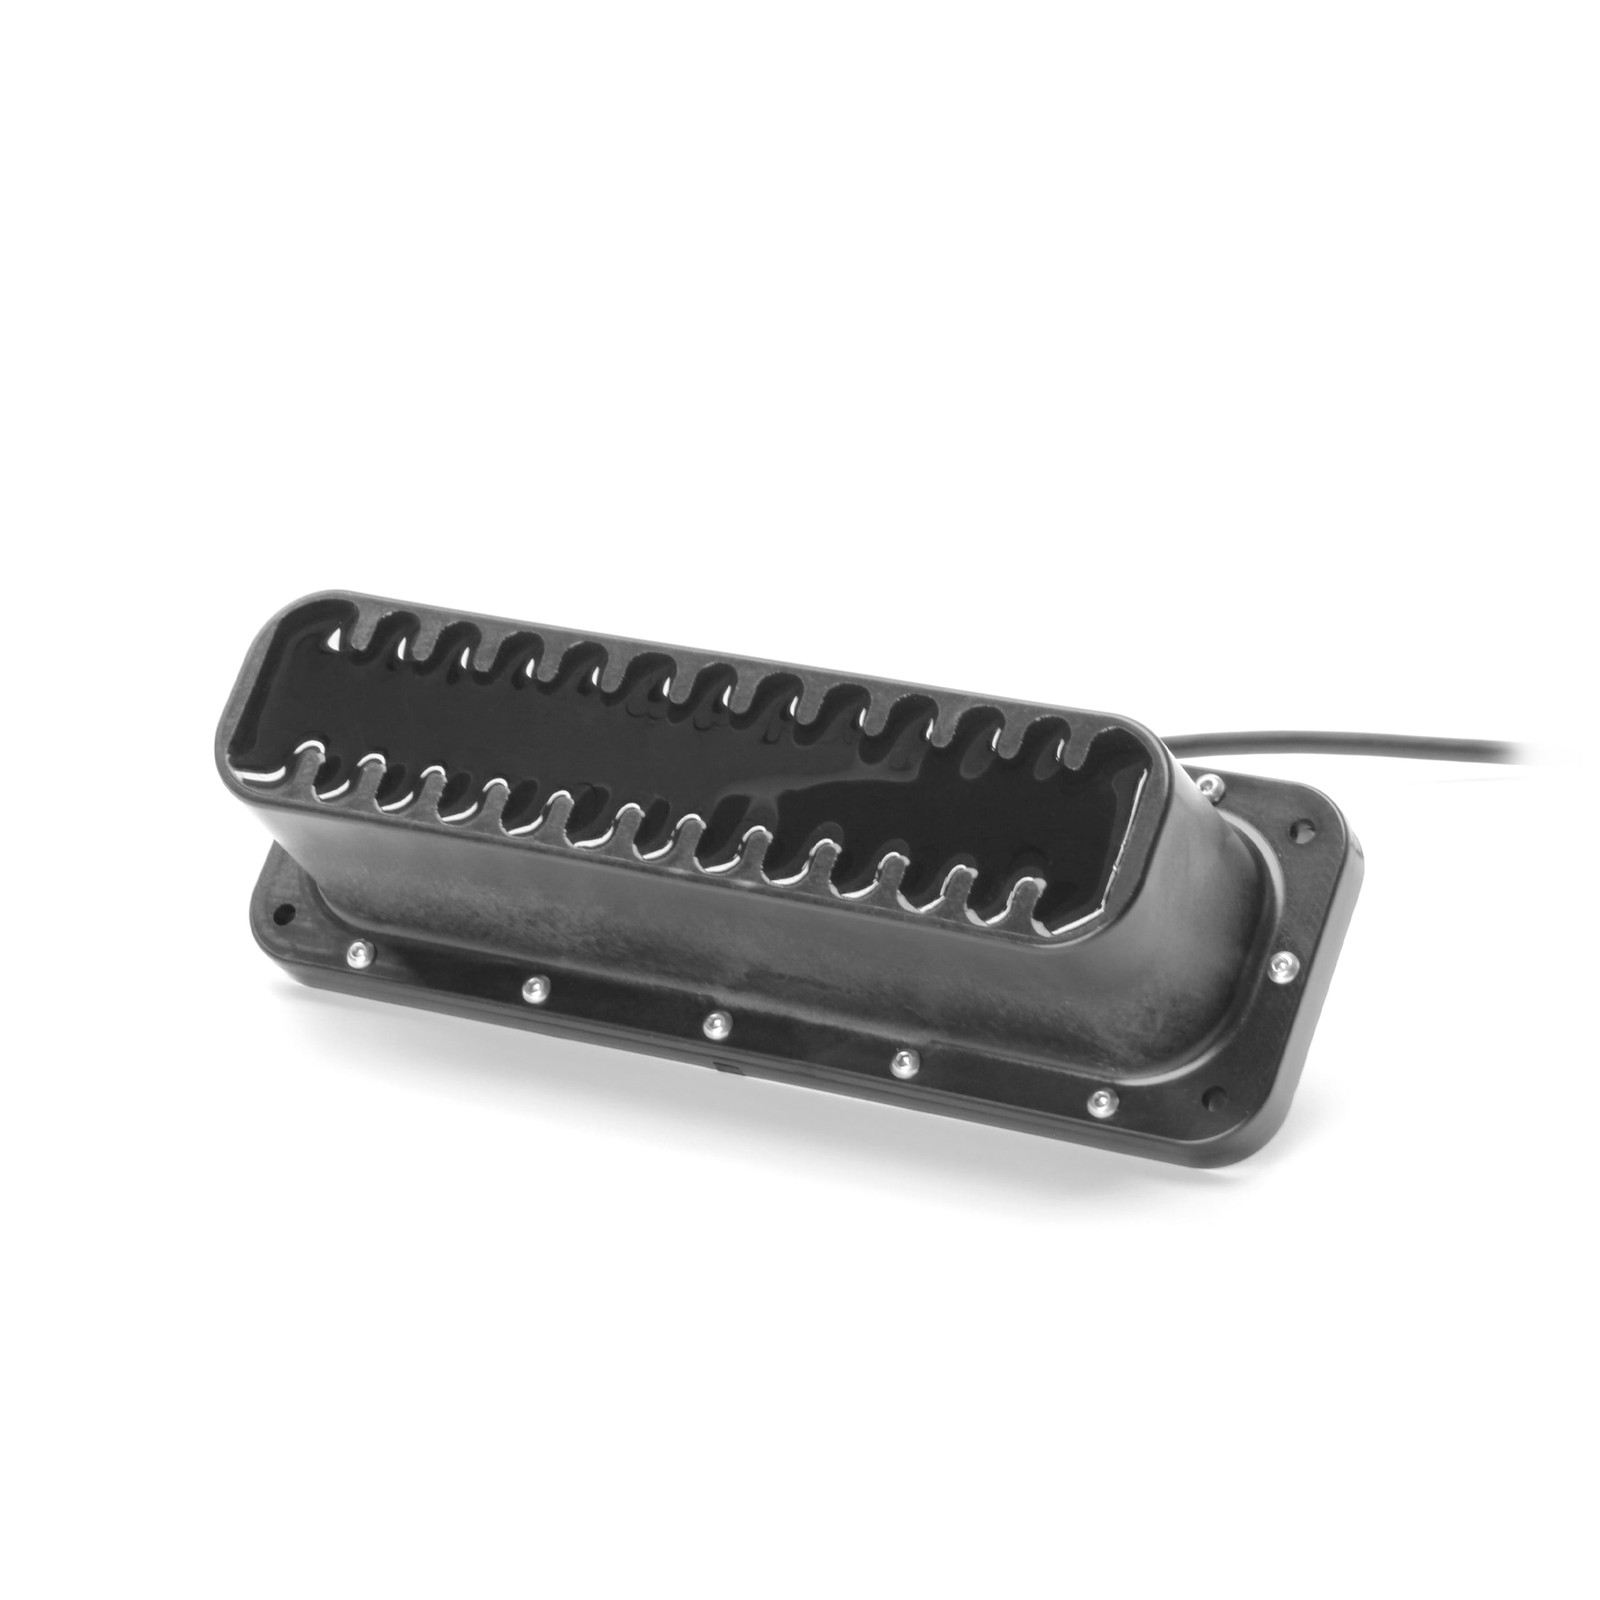
\includegraphics[height=1.25cm, keepaspectratio]{cerulean_omniscan.jpg} &
      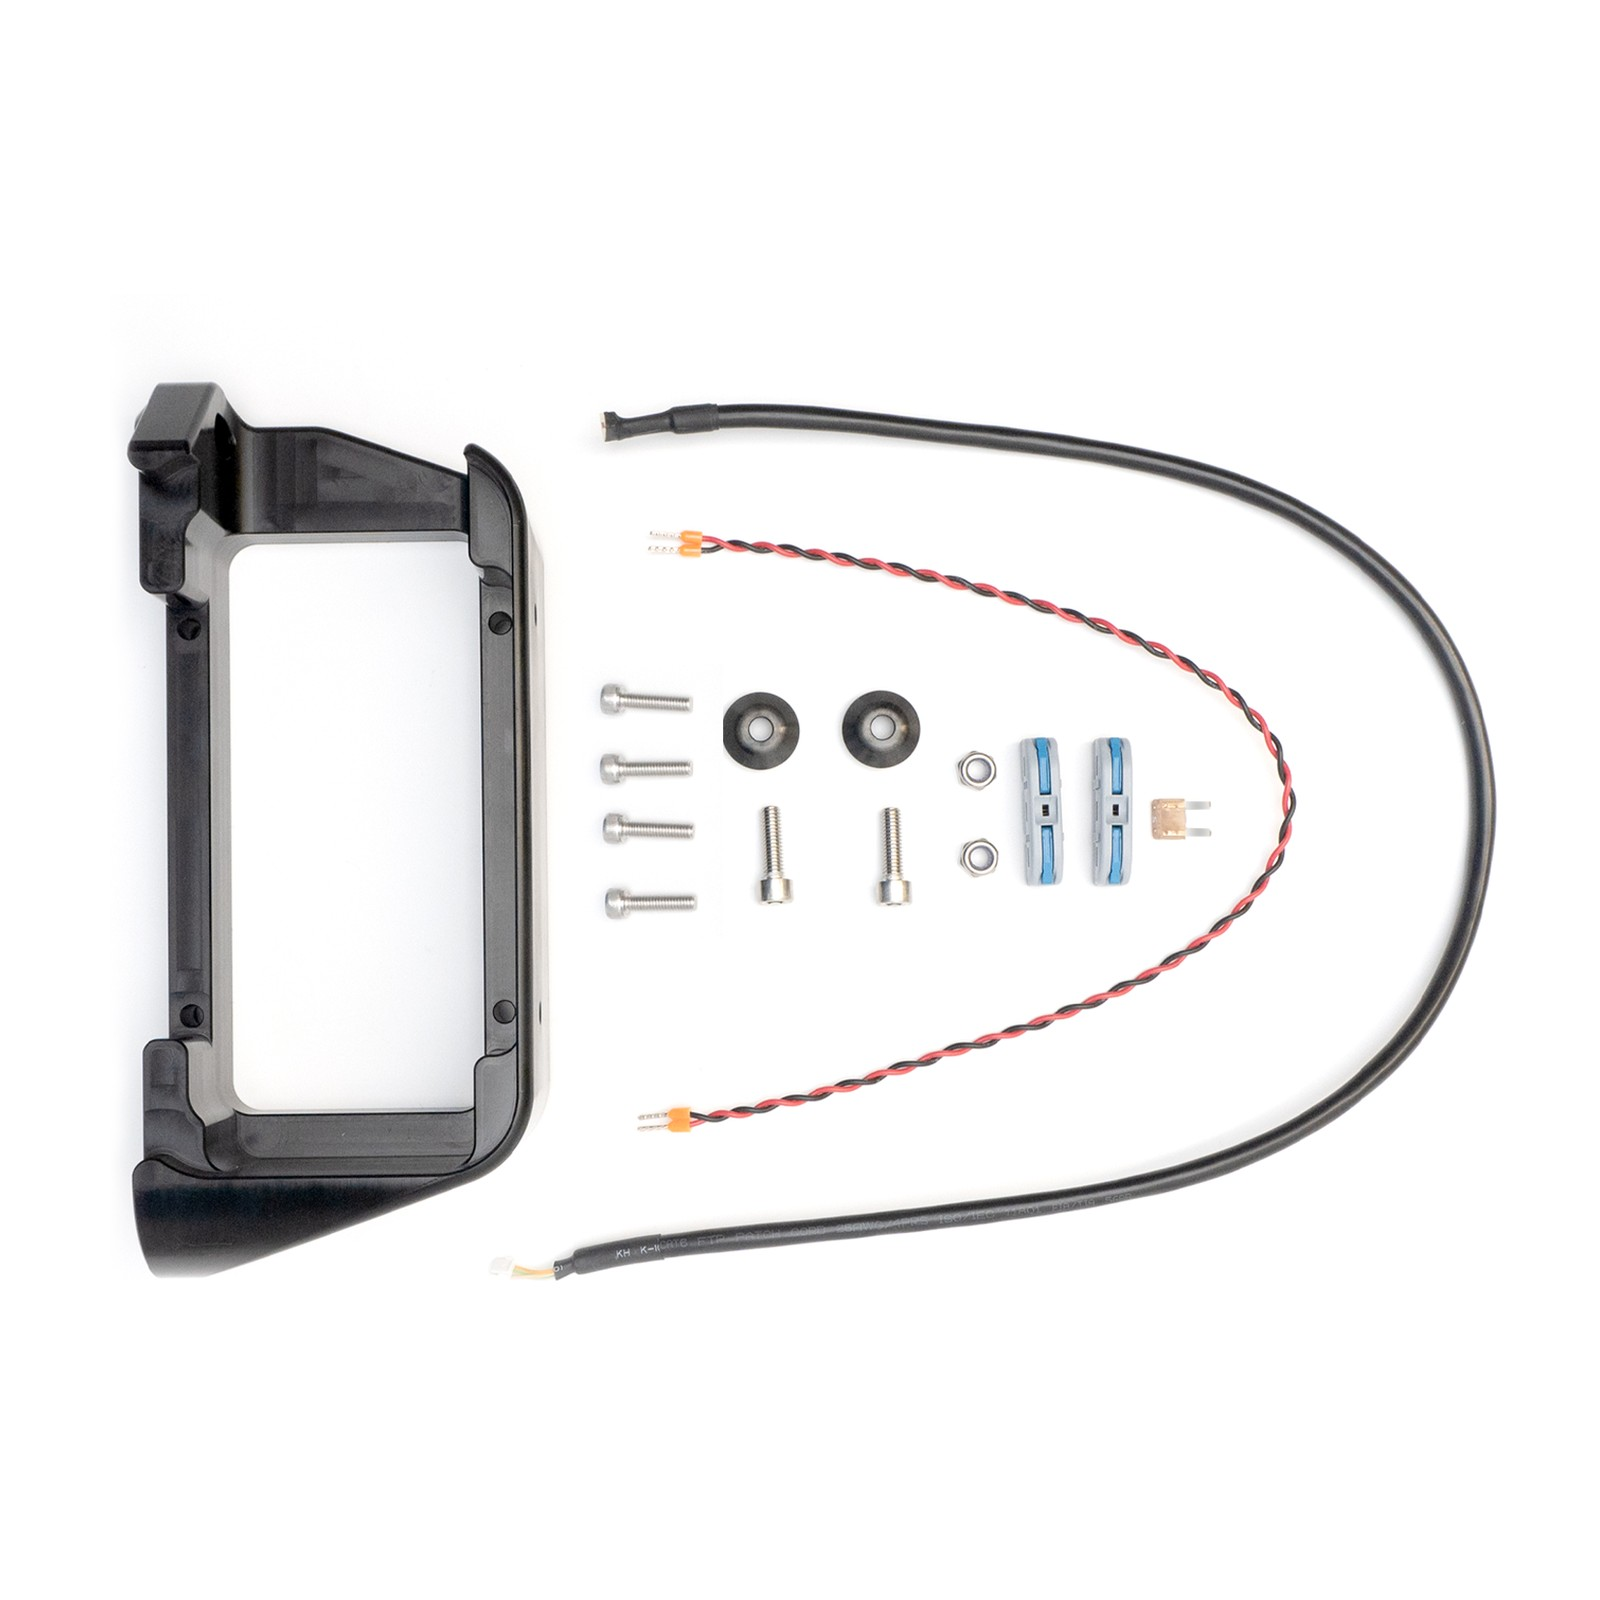
\includegraphics[height=1.25cm, keepaspectratio]{cerulean_surveyor_mbes.jpg} \\
      \textbf{Omniscan 450 FS} &
      \textbf{MBES Surveyor 240-16}
    \end{tabular}%
    }
  \end{center}
  \scriptsize
  \begin{itemize}
    \item \textbf{Ping Sonar (115 kHz)} : échosondeur monofaisceau ($0.5\text{--}50\,\text{m}$), altimètre ROV et bathymétrie BlueBoat.
    \item \textbf{Ping360 (750 kHz)} : sonar à balayage mécanique $360^\circ$ pour navigation et détection d'obstacles en eau turbide.
    \item \textbf{Cerulean Omniscan 450 FS} : sonar d'imagerie acoustique 2D haute résolution pour inspection de parois et navigation.
    \item \textbf{Cerulean Surveyor 240-16 (MBES)} : sondeur multifaisceaux 16 récepteurs pour bathymétrie fauchée 3D haute densité sur BlueBoat.
  \end{itemize}
\end{tcolorbox}

% BLOC 9 : LOCALISATION SOUS-MARINE & ACOUSTIQUE
\begin{tcolorbox}[title={9. Localisation Sous-Marine : Estime, DVL, LBL/USBL \& Propagation}]
  \begin{center}
    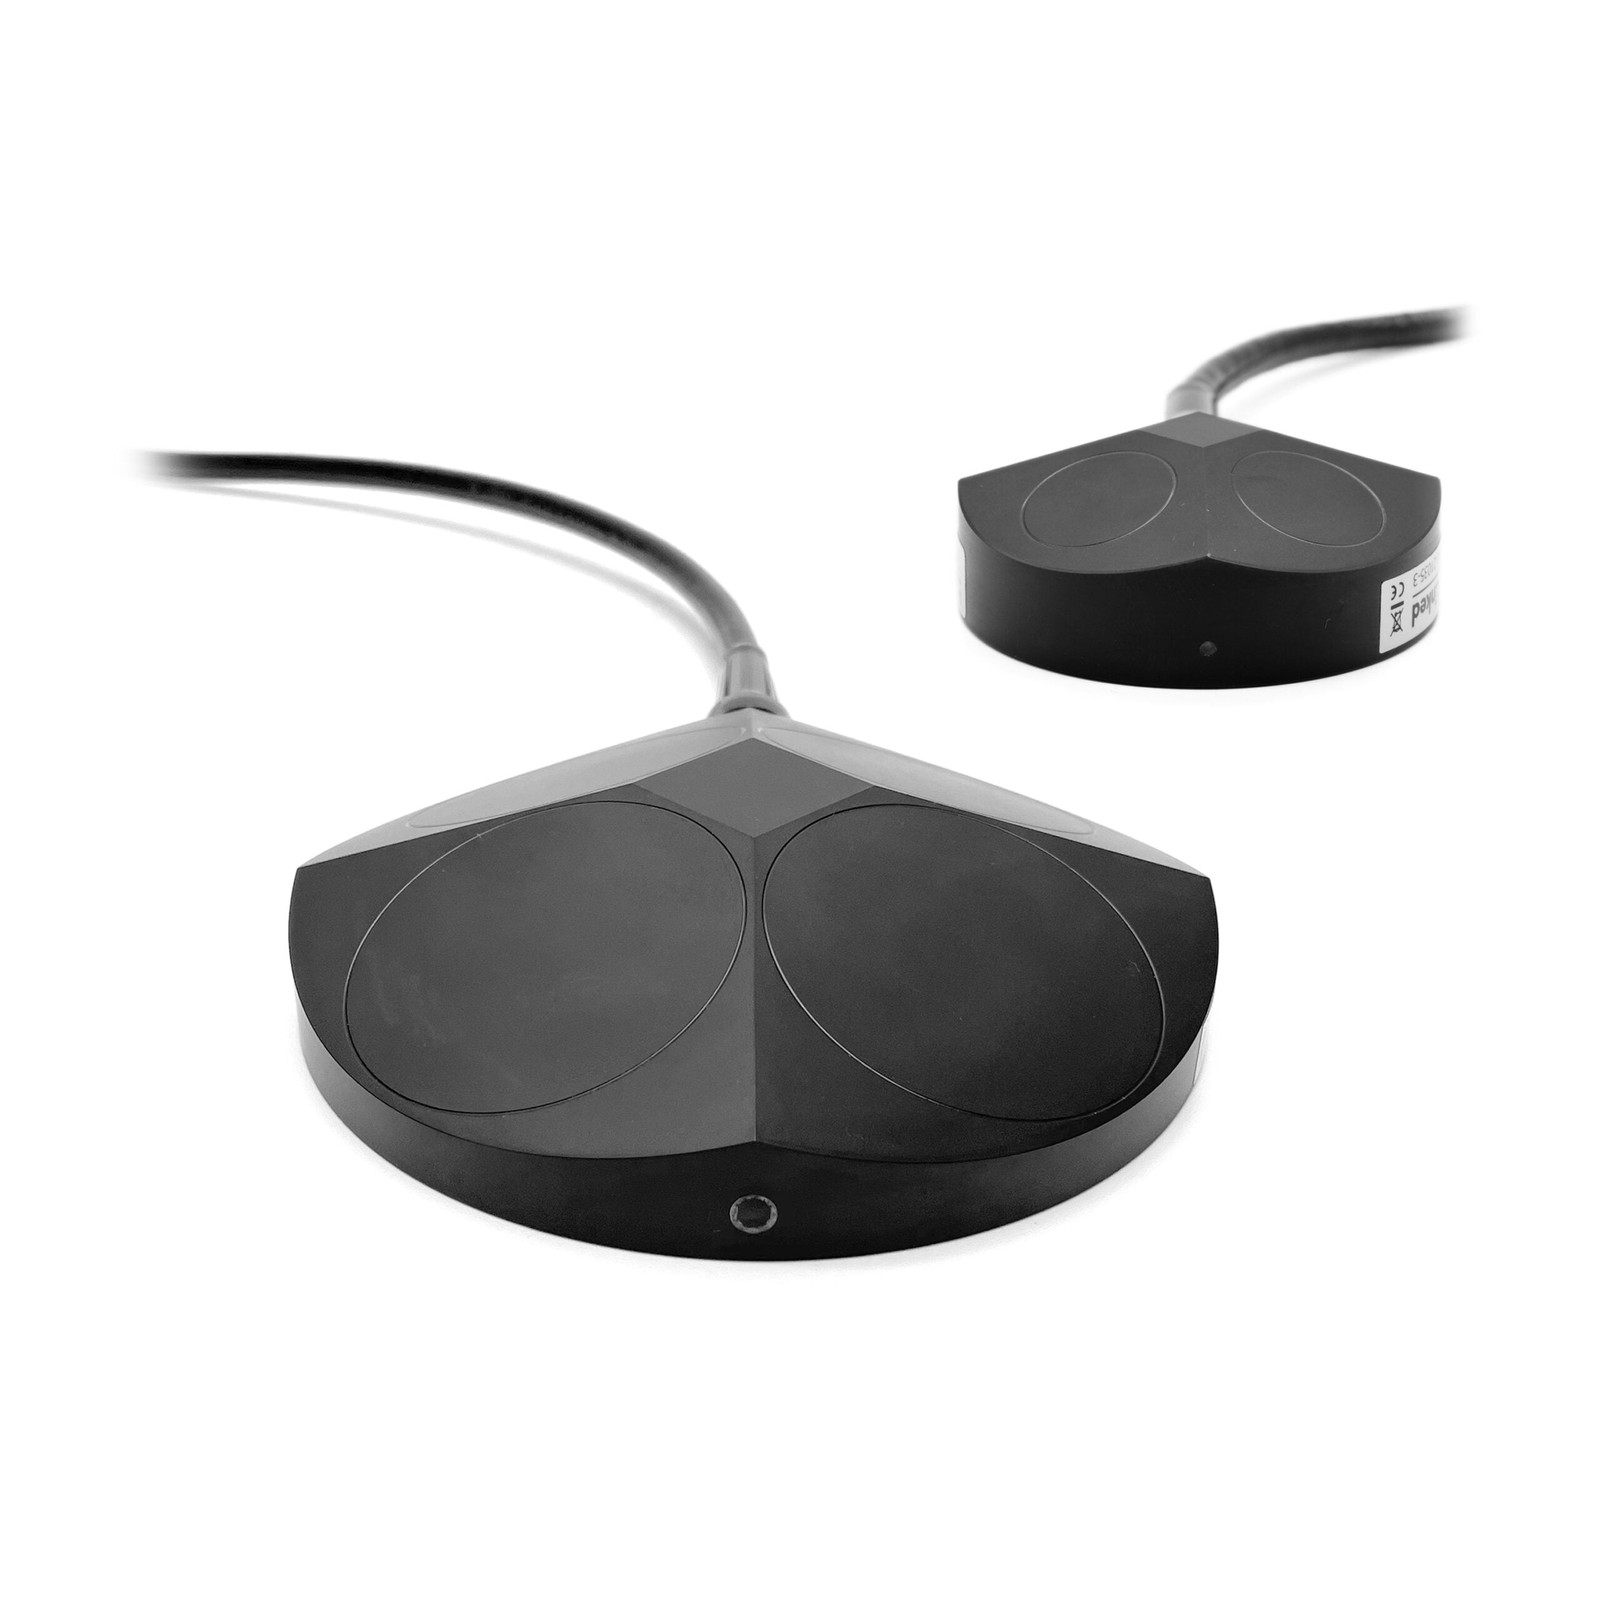
\includegraphics[height=1.2cm, keepaspectratio]{dvl_a50.jpg}\\
    \tiny\textbf{DVL-A50 (Odométrie fond Janus 1 MHz, 270 g)}
  \end{center}
  \scriptsize
  \begin{itemize}
    \item \textbf{Fix Surface \& Dead Reckoning} : GNSS absorbé à l'immersion ($\delta \approx 6\,\text{mm}$). Dernier fix en surface ($t_0$) puis intégration à l'estime.
    \item \textbf{Dérive Inéluctable IMU} : gyros $\rightarrow$ dérive angulaire $\propto t$ ; accéléros $\rightarrow$ \alertw{dérive quadratique $\propto \frac{1}{2} a_{\text{drift}} t^2$} ($>1\,\text{km}$ en 10 min !). Axe $Z$ parfaitement borné par le Bar30.
    \item \textbf{DVL (Doppler Velocity Log)} : mesure la vitesse sol 3D. Intégration simple $\rightarrow$ dérive bornée à \succw{$\mathbf{0.2\%}$ de la distance}.
    \item \textbf{Positionnement Absolu (LBL vs USBL)} :
      \begin{itemize}\scriptsize
        \item \textbf{LBL (Long BaseLine)} : 3--4 balises au fond, triangulation ToF, précision centimétrique fixe, logistique très lourde.
        \item \textbf{USBL (Ultra-Short BaseLine)} : 1 antenne sous le bateau/ASV, ToF + déphasage, précision $0.5\text{--}1\%$ portée, mobile, zéro matériel au fond.
      \end{itemize}
    \item \succw{USBL Low-Cost ($\approx \mathbf{5\text{--}8\,\text{k€}}$) \& Modem} : (ex: Water Linked) combine tracking et \textbf{télémétrie acoustique (quelques kB/s)} : alarmes, état Li-ion, consignes.
    \item \alertw{Pièges de Propagation Acoustique} :
      \begin{itemize}\scriptsize
        \item \textit{Réfraction $c(z)$} : thermocline courbe les rayons $\rightarrow$ zones d'ombre.
        \item \textit{Multi-trajets} : échos surface/fond brouillant par petits fonds ($<15\,\text{m}$).
        \item \textit{Masquage} : roches, épaves, bulles d'air sous coque (*wake*).
      \end{itemize}
  \end{itemize}
\end{tcolorbox}

\columnbreak

% BLOC 10 : ARCHITECTURE DES ESSAIS ET POSTE DE SURFACE
\begin{tcolorbox}[title={10. Architecture Essais : Station Sol, FXTI, BaseStation \& RC}]
  \begin{center}
    \resizebox{\linewidth}{!}{%
    \begin{tabular}{cc}
      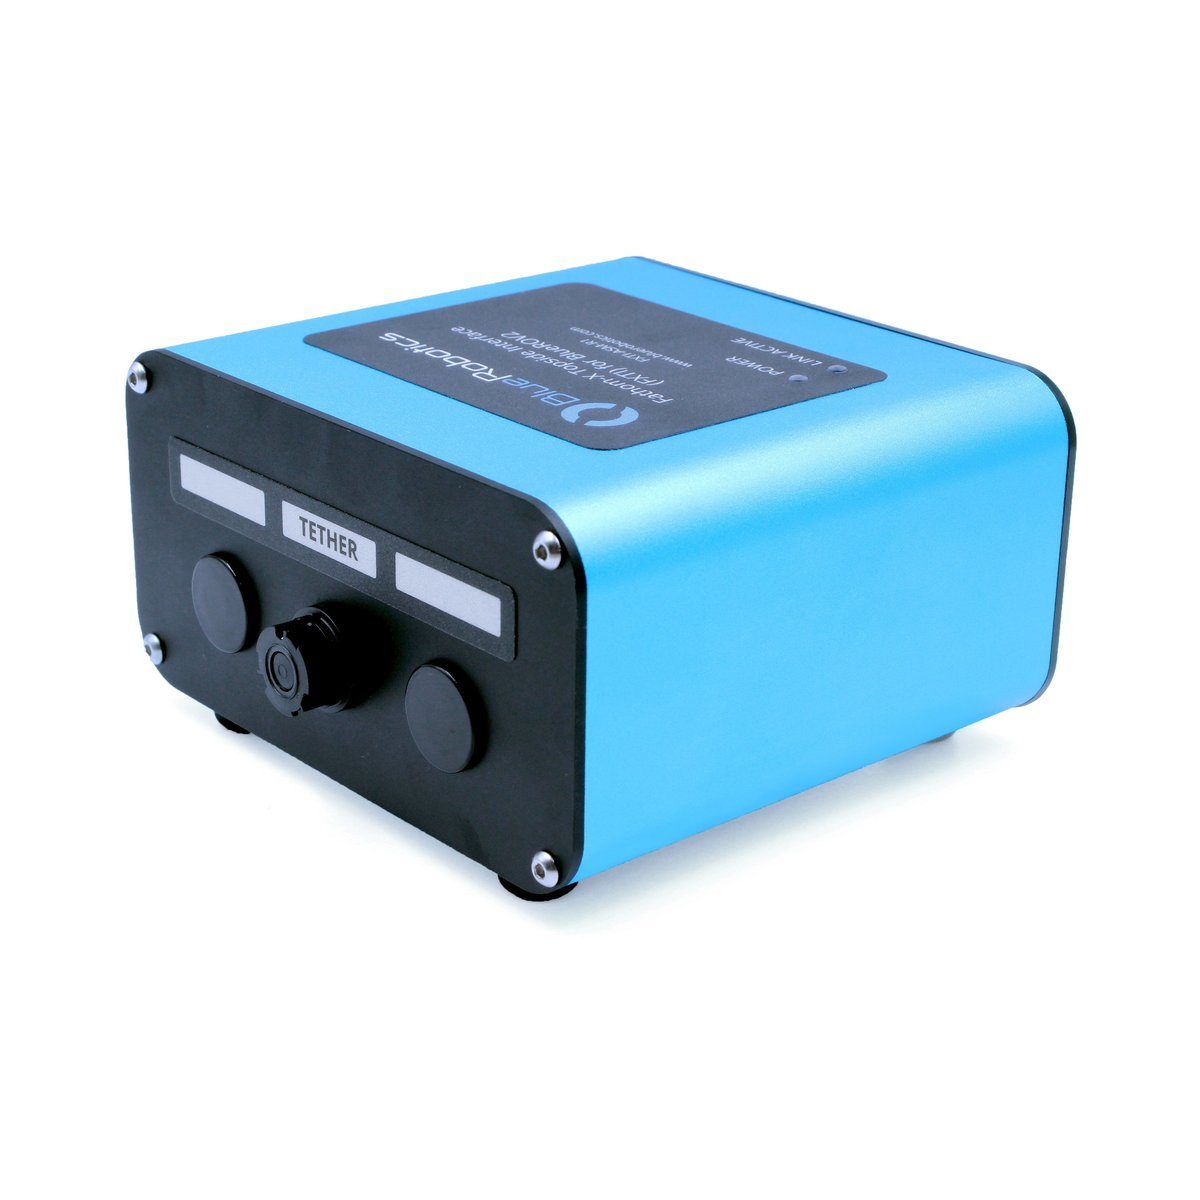
\includegraphics[height=1.35cm, keepaspectratio]{fxti_interface.jpg} &
      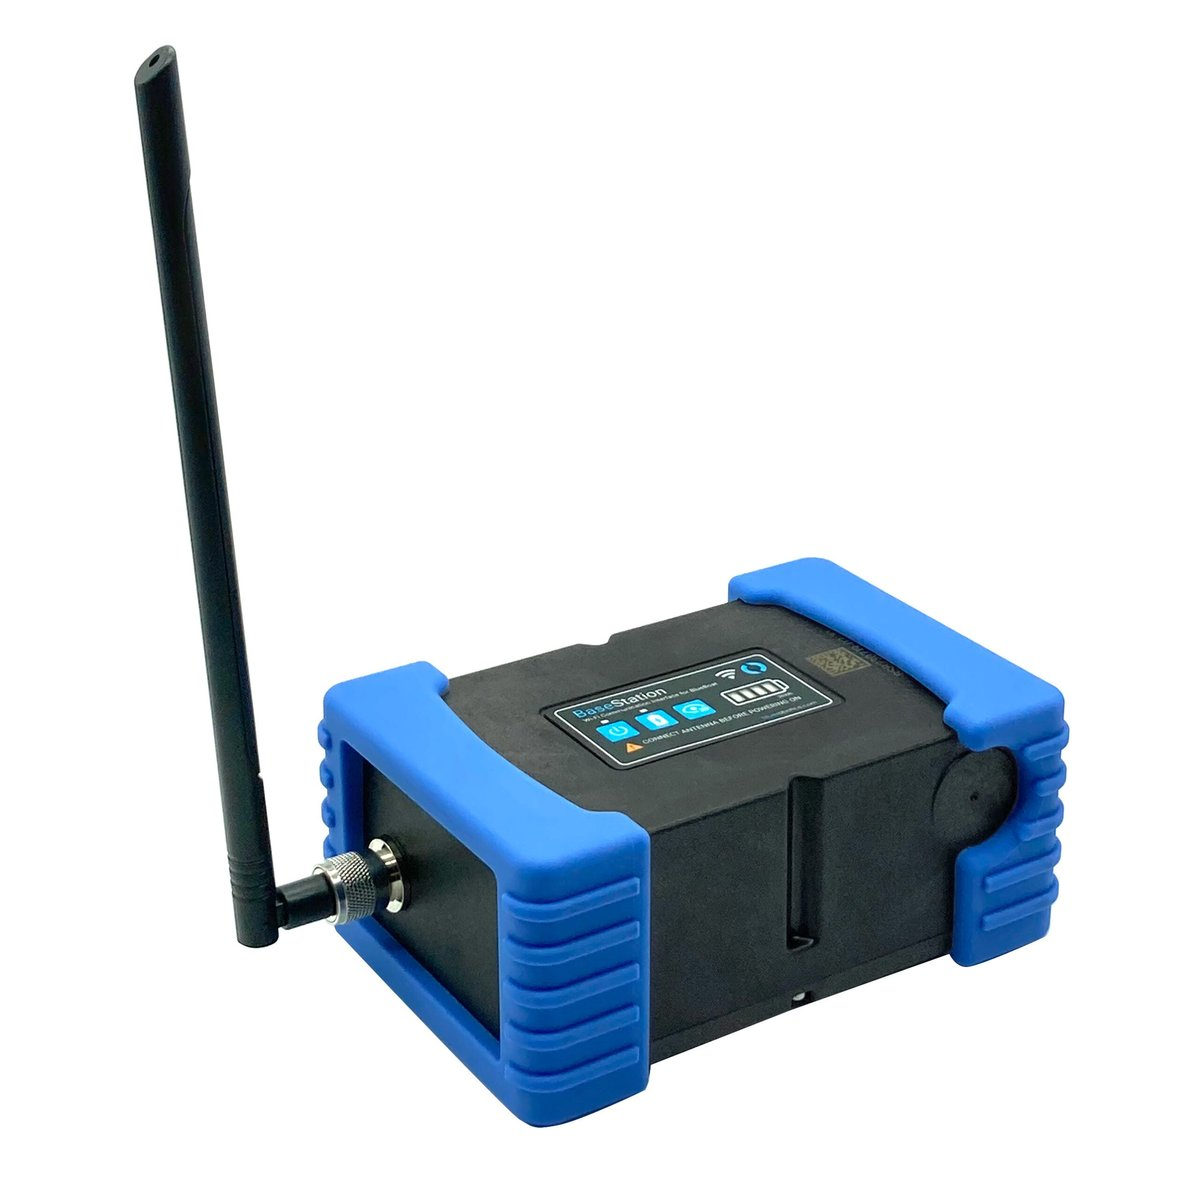
\includegraphics[height=1.35cm, keepaspectratio]{basestation_wifi.jpg} \\
      \textbf{Boîtier FXTI (Ombilical ROV)} &
      \textbf{BaseStation WiFi 2.4 GHz (ASV)}
    \end{tabular}%
    }
  \end{center}
  \scriptsize
  \begin{itemize}
    \item \textbf{Station Sol (GCS)} : PC avec \textbf{QGroundControl} ou navigateur web \textbf{Cockpit} (interface modulaire HTML5/Vue.js sous BlueOS).
    \item \textbf{Liaison Filaire ROV (FXTI \& Tether)} : convertit l'ombilical Fathom (Standard $\varnothing 7.6\,\text{mm}$ ou Slim $\varnothing 4.0\,\text{mm}$) via CPL HomePlug AV ($100\,\text{Mbps}$). Enrouleur avec collecteur tournant (*slip ring*) anti-vrille.
    \item \textbf{Liaison Surface ASV (BaseStation)} : antenne WiFi MikroTik 2.4 GHz longue portée ($>1\,\text{km}$) sur mât pour communiquer avec le BlueBoat.
    \item \textbf{Radiocommande RC manuelle (2.4 GHz SBUS)} : récepteur RC relié au Navigator. \succw{Indispensable pour la mise à l'eau} et récupération au quai, et arrêt d'urgence matériel indépendant du PC/WiFi !
  \end{itemize}
\end{tcolorbox}

% BLOC 11 : ALIMENTATION HAUTE TENSION OTPS & DONNEES FAIR
\begin{tcolorbox}[title={11. Alimentation Haute Tension (OTPS) \& Données FAIR}]
  \begin{center}
    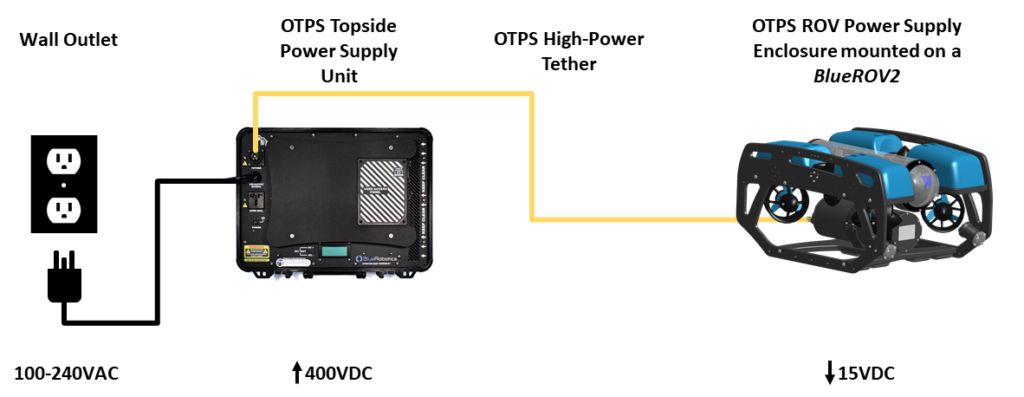
\includegraphics[height=1.15cm, keepaspectratio]{otps_power_system.png}\\
    \tiny\textbf{Système OTPS : 400V DC surface $\rightarrow$ abaissement 15V DC ($1000\,\text{W}$) sous-marin}
  \end{center}
  \scriptsize
  \begin{itemize}
    \item \textbf{Principe OTPS (Outland Technology Power Supply)} : pour plonger 24h/24 sans batterie, la surface élève le secteur à \succw{$\mathbf{400\,\text{V DC}}$}. À puissance égale ($1000\,\text{W}$), le courant passe de $67\,\text{A}$ ($15\,\text{V}$) à seulement $\mathbf{2.5\,\text{A}}$ !
    \item \textbf{Carte sous-marine de transformation} : hacheur abaisseur DC-DC haute puissance dans le caisson ROV convertissant le 400V DC en \textbf{$15\,\text{V DC}$ (jusqu'à $45\,\text{A}$)} régulé avec isolation galvanique.
    \item \textbf{Formats FAIR} : enregistrements \code{rosbag2} (.mcap), grilles bathymétriques GeoTIFF et profils CTD \textbf{NetCDF-4} avec métadonnées CF.
  \end{itemize}
\end{tcolorbox}

% BLOC 12 : REGLEMENTATION DRONES MARINS & PING
\begin{tcolorbox}[title={12. Réglementation Drone Maritime (\href{https://www.legifrance.gouv.fr/jorf/id/JORFTEXT000049583905}{\underline{Décret 2024-461}}) \& PING}]
  \scriptsize
  \begin{itemize}
    \item \textbf{Seuils Drone (\href{https://www.legifrance.gouv.fr/codes/article_lc/LEGIARTI000049585210}{\underline{Art. R. 5000-1}})} : flottant/sous-marin sans équipage : $1\,\text{m} < L_{\text{HT}} < 16\,\text{m}$, vitesse $\le 20\,\text{kn}$, énergie $<300\,\text{kJ}$, jauge $<100$ UMS.
    \item \textbf{Capitaine 200 obligatoire} : en mer ouverte (mission pro/recherche), la responsabilité nautique RIPAM (COLREG 72) impose un marin breveté \alertw{Capitaine 200} sur le navire support ou au centre de télé-opération (COD).
    \item \textbf{Astuces \& Dérogations Labo} :
      (1) \succw{ROV filaire captif} = équipement immergé sous garde du bateau (zéro qualification drone requise) ;
      (2) \succw{Engins $\le 1\,\text{m}$} = hors champ R. 5000-1 (modélisme/outil léger) ;
      (3) \succw{Bande des 300 m \& lacs} = police du maire / eaux intérieures VNF.
    \item \textbf{Plateforme PING} (\href{https://portail.ping-info-nautique.fr/}{\underline{portail.ping-info-nautique.fr}}) : consultation obligatoire des AVURNAV, zones militaires, parcs marins et chenaux.
  \end{itemize}
\end{tcolorbox}

% BLOC 13 : REGLES D'OR APRES MISSION
\begin{tcolorbox}[title={13. Règles d'Or : Après Récupération}]
  \scriptsize
  \begin{enumerate}
    \item \textbf{Rinçage immédiat à l'eau douce} : moteurs T200 30s en bac d'eau douce (chasser le sel des paliers PEEK).
    \item \textbf{Séchage externe intégral} avant toute ouverture de caisson étanche (zéro goutte tolérée).
    \item \textbf{Inspection anode sacrificielle} en zinc et \textbf{double sauvegarde} des données scientifiques.
    \item Stockage des batteries Li-ion à tension de stockage ($3.85\,\text{V/cellule}$) en caisse ignifugée.
  \end{enumerate}
\end{tcolorbox}

\end{multicols}

\vspace{-6pt}
\begin{center}
  \scriptsize\textcolor{gray}{Mémento ANF ArchiDrone 2026 --- Réseaux Drone\&Cap' \& 2RM --- Guide de terrain conçu pour la recherche scientifique marine.}
\end{center}

\end{document}
